\chapter[Directional detection]{Velocity parametrisation for directional experiments}
\label{ch:directional}

While many direct detection experiments seek to measure the recoil energies deposited by weakly interacting massive particles (WIMPs) scattering off detector nuclei, \textit{directional} experiments aim to measure both the energy and direction of the recoil. While the recoil distribution of typical backgrounds is expected to be roughly isotropic, the WIMP-induced recoil distribution is expected to be highly directional \cite{Spergel:1988}. The motion of the Sun through the Galactic dark matter (DM) halo generates a so-called `WIMP wind', leading to an event rate peaked in the opposing direction, the direction of the constellation Cygnus.\footnote{In fact, for high mass WIMPs and low energy recoils, the event rate may be peaked in a ring around the direction of Cygnus \cite{Bozorgnia:2011}.}

The ability of directional detection to distinguish background from signal and to provide a model independent confirmation of the dark matter origin of the signal make it a promising search strategy. The directional signature of the WIMP signal may also allow it to be distinguished from neutrino scattering, allowing directional detectors to probe below the neutrino floor \cite{Grothaus:2014}. However, measuring the direction of rare, low energy recoils remains challenging. A number of directional detectors are currently in development and a number of novel methods for directional detection have also been proposed.

Measuring the directional recoil spectrum allows us to probe not just the energy distribution of WIMPs in the Galactic halo (embodied in the speed distribution $f_1(v)$), but the full 3-dimensional velocity distribution $f(\textbf{v})$. This may allow us to gain new insight into the phase space distribution of the Milky Way's DM halo. This should in turn allow us to test the results of N-body simulations and to probe the process of structure formation on galactic scales. However, directionality also introduces new uncertainties into calculating the event rate. While non-directional detection leaves us with a single free function in the form of $f_1(v)$, the directional case relies upon the \textit{a priori} unknown function of a 3-dimensional vector, $f(\textbf{v})$.

In this chapter, we will first introduce the formalism by which the directional rate is calculated. Specifically, we introduce the Radon transform which relates the WIMP velocity distribution to the corresponding nuclear recoil distribution.  We then discuss the current state of directional detection technology and the progress of several directional experiments. We the summarise previous approaches to mitigating the uncertainties associated with the velocity distribution. Finally, we consider a new method for parametrising $f(\textbf{v})$, which allows it to be written in terms of a finite number of one-dimensional functions, and how to calculate the Radon transform of this new, discretised distribution function.




\section{Directional event rate}

We wish to calculate the directional event spectrum in a dark matter detector. We follow the treatment of Gondolo \cite{Gondolo:2002}, noting that similar calculations were performed previously by Copi, Heo and Krauss \cite{Copi:1999} and later by Copi and Krauss \cite{Copi:2001}. The scattering of a WIMP with a nucleus is illustrated in Fig.~\ref{fig:directional:scattering}.

\begin{figure}[h!]
  \centering
  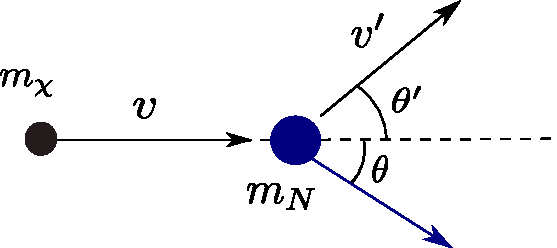
\includegraphics[width=0.75\textwidth]{Directional/Scattering.pdf}
\caption[Illustration of DM-nucleus scattering]{Illustration of the scattering of a DM particle of mass $m_\chi$ from a nucleus of mass $m_N$.}
  \label{fig:directional:scattering}
\end{figure}

We consider a DM particle of mass \(m_\chi\) impinging with velocity \(\textbf{v} = v\left(1,0\right)\) on a stationary target nucleus of mass \(m_N\), where we have suppressed the azimuthal dimension. The dark matter scatters with velocity \(\textbf{v}' = v'\left(\cos \theta',\sin \theta'\right)\) and the nucleus has final momentum \(\textbf{q} = q\left(\cos \theta, \sin \theta\right)\). From conservation of linear momentum we obtain:

\begin{align}
m_\chi v' \cos \theta' &= m_\chi v - q\cos \theta \,, \label{eq:momentumx}\\
m_\chi v' \sin \theta' &= q \sin \theta \,. \label{eq:momentumy}
\end{align}
We can eliminate \(\theta'\) by summing the squares of Eqs. \ref{eq:momentumx} and \ref{eq:momentumy}, to obtain:

\begin{equation}
v'^2 = v^2 - \frac{2 v q \cos \theta}{m_\chi} + \frac{q^2}{m_\chi^2}\,.
\end{equation}
From energy conservation, we obtain:

\begin{equation}
\label{eq:Energy}
v'^2 = v^2 - \frac{q^2}{m_\chi m_N} \,.
\end{equation}
Combining these, we see that the recoil momentum of the target nucleus is given by

\begin{equation}
\label{eq:constraint}
q = 2\mu_{\chi N} v \cos \theta \,,
\end{equation}
where \(\mu_{\chi N} = m_\chi m_N/(m_\chi + m_N)\) is the DM-nucleus reduced mass.


For a WIMP-nucleus interaction cross section which is independent of velocity, we can write the differential cross section as

\begin{equation}
\frac{\textrm{d}\sigma}{\textrm{d}E_R} = \frac{m_N \sigma_p}{2 \mu_{\chi p}^2 v^2} \mathcal{C} F^2(E_R)\,,
\end{equation}
where \(E_R\) is the nuclear recoil energy, \(\sigma_p\) is the WIMP-proton interaction cross section (which may be spin-dependent (SD) or spin-independent (SI)) and $\mathcal{C}$ and $F^2$ are the corresponding enhancement factor and nuclear form factor (see Eq.~\ref{eq:DD:fullsigma}). We then require a Dirac \(\delta\)-function to impose the condition in Eq.\ \ref{eq:constraint}:

\begin{equation}
\frac{\textrm{d}\sigma}{\textrm{d}E_R\textrm{d}\cos\theta} = \frac{m_N \sigma_p}{2 \mu_{\chi p}^2 v^2} \mathcal{C} F^2(E_R) \delta\left(\cos\theta - q/2\mu_{\chi N}v\right)\,.
\end{equation}
The collision is azimuthally symmetric, so that \(\textrm{d}\Omega_q = 2\pi\,\textrm{d}\cos\theta\). Rewriting the $\delta$-function as
\begin{equation}
 \delta\left(\cos\theta - q/2\mu_{\chi N}v\right) = v \delta\left(v \cos\theta - q/2\mu_{\chi N}\right)\,,
\end{equation}
we obtain the double differential cross-section \(\textrm{d}\sigma/\textrm{d}E_R \textrm{d}\Omega_q\):

\begin{equation}
\frac{\textrm{d}\sigma}{\textrm{d}E_R \textrm{d}\Omega_q} = \frac{m_N \sigma_p}{4\pi\mu_{\chi p}^2v} \mathcal{C} F^2(E_R) \delta\left(v \cos\theta - v_\textrm{min}\right)\,,
\end{equation}
where \(v_\textrm{min}\) is the minimum WIMP speed required to excite a recoil of momentum \(q\) or, equivalently, energy \(E_R\):


\begin{equation}
v_\textrm{min} = \frac{q}{2\mu_{\chi N}} = \sqrt{\frac{m_N E_R}{2\mu_{\chi N}^2}}\,.
\end{equation}

To obtain the differential rate per unit detector mass, we divide by the mass of the target nucleus and multiply by the WIMP flux at velocity \(\textbf{v}\),

\begin{equation}
\frac{\rho_0}{m_\chi} v f(\textbf{v}) \, \textrm{d}^3 \textbf{v}\,,
\end{equation}
where \(\rho_0\) is the local dark matter mass density, before integrating over all velocities. Combining these, we obtain:

\begin{equation}
\frac{\textrm{d}R}{\textrm{d}E_R \textrm{d}\Omega_q} = \frac{\rho_0 \sigma_p}{4\pi \mu_{\chi p}^2 m_\chi} \mathcal{C} F^2(E_R) \hat{f}\left(v_\textrm{min},\hat{\textbf{q}}\right)\,,
\end{equation}
where \(\hat{f}\left(v_\textrm{min},\hat{\textbf{q}}\right)\) is the Radon Transform of the velocity distribution, defined as:

\begin{equation}
\hat{f}\left(v_\textrm{min},\hat{\textbf{q}}\right) = \int \delta\left(v_\textrm{min} - \textbf{v}\cdot\hat{\textbf{q}}\right) f(\textbf{v}) \,\textrm{d}^3\textbf{v}\,.
\end{equation}
Geometrically, this is the integral of \(f(\textbf{v})\) over a plane perpendicular to \(\hat{\textbf{q}}\) at a distance \(v_\textrm{min}\) from the origin. In physical terms, for a given recoil angle and energy, we integrate over all WIMP velocities satisfying the kinematic constraint given by Eq.\ \ref{eq:constraint}.

\subsection{Examples}

We consider several examples of velocity distributions and their corresponding Radon transforms. For an isotropic Maxwell-Boltzmann distribution with dispersion $\sigma_v$,

\begin{equation}
f(\textbf{v}) = \frac{1}{(2\pi \sigma_v^2)^{\frac{3}{2}}} \exp \left[ -\frac{\textbf{v}^2}{2 \sigma_v^2}\right]\,,
\end{equation}
the Radon transform is also isotropic,
\begin{equation}
\hat{f}(\vmin,\hat{\textbf{q}}) = \frac{1}{(2\pi \sigma_v^2)^{\frac{1}{2}}} \exp \left[ -\frac{\vmin^2}{2 \sigma_v^2}\right]\,.
\end{equation}
If we take this form to describe the DM velocity distribution in the Galactic frame, we must transform to the laboratory frame using the relation \cite{Gondolo:2002}

\begin{equation}
\hat{f}_\textrm{lab}(\vmin, \hat{\textbf{q}}) = \hat{f}_\textrm{gal}(\vmin - \textbf{v}_\textrm{lag}\cdot\hat{\textbf{q}} , \hat{\textbf{q}})\,,
\end{equation}
where $\textbf{v}_\textrm{lag}$ is the velocity of the peak of the Galactic distribution with respect to the laboratory. We therefore obtain the Radon transform of the Standard Halo Model (SHM):

\begin{equation}
\label{eq:directional:SHM}
\hat{f}(\vmin,\hat{\textbf{q}}) =  \frac{1}{(2\pi \sigma_v^2)^{\frac{1}{2}}} \exp \left[ -\frac{(\vmin - \textbf{v}_\textrm{lag}\cdot\hat{\textbf{q}})^2}{2 \sigma_v^2}\right]\,.
\end{equation}
This can be extended to incorporate a cut off at the Galactic escape speed, or to more general anisotropic velocity distributions \cite{Gondolo:2002}.

Another interesting velocity distribution is that of a stream

\begin{equation}
f(\textbf{v}) = \delta(\textbf{v} - \textbf{v}_s)\,,
\end{equation}
which has Radon transform

\begin{equation}
\hat{f}(\vmin,\hat{\textbf{q}}) =  \delta(\vmin - \textbf{v}_\textrm{lag}\cdot\hat{\textbf{q}})\,.
\end{equation}
This results in a highly directional signal, producing a spherical recoil spectrum centred on $\textbf{v} = \textbf{v}_s/2$.


In Fig.~\ref{fig:directional:Radon}, we illustrate the Radon transform of the SHM (top), the SHM with a 23\% contribution from a dark disk (middle), and a stream (bottom) with $v_\textrm{lag} = 400 \kms$. In each case, we have integrated over the $\phi$ direction and show $\hat{f}(v, \cos\theta)$. In the case of the SHM and the stream, there is a clear anisotropy and the two scenarios should be easily distinguishable. This highlights the discriminatory power of directional detection. It has previously been demonstrated that only of order 10 events would be required to distinguish a directional WIMP signal from an isotropic background. Furthermore, with of order 100 events, it should be possible to detect a deviation in peak recoil direction due to a stream \cite{Morgan:2005} (though this depends on the density and velocity of the stream). In the case of the SHM with a dark disk contribution, the spectrum is more isotropic. This is because the Radon transform is dominated by the dark disk contribution, which has a lower value of $v_\textrm{lag} = 50 \kms$ and therefore appears more isotropic in the Earth frame.

\begin{figure}[pht!]
  \centering
  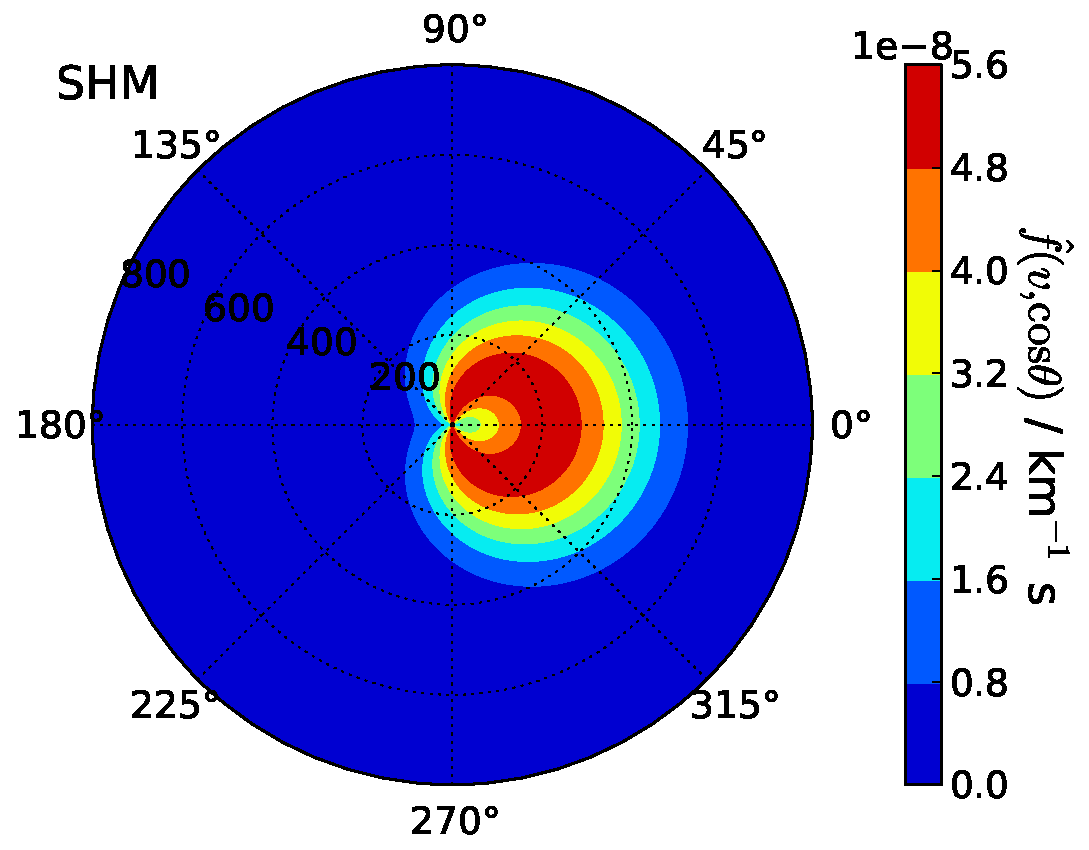
\includegraphics[width=0.75\textwidth]{Directional/SHMRadonpolar.pdf}
  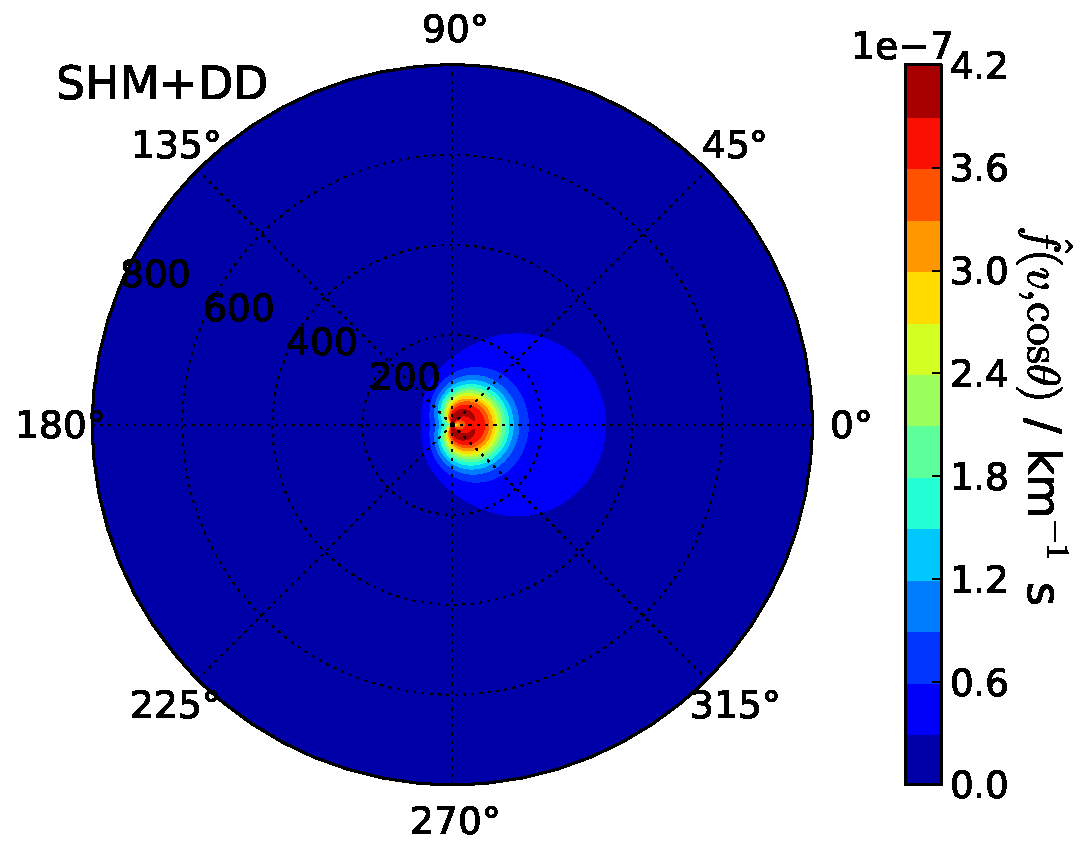
\includegraphics[width=0.75\textwidth]{Directional/SHMDDRadonpolar.pdf}

  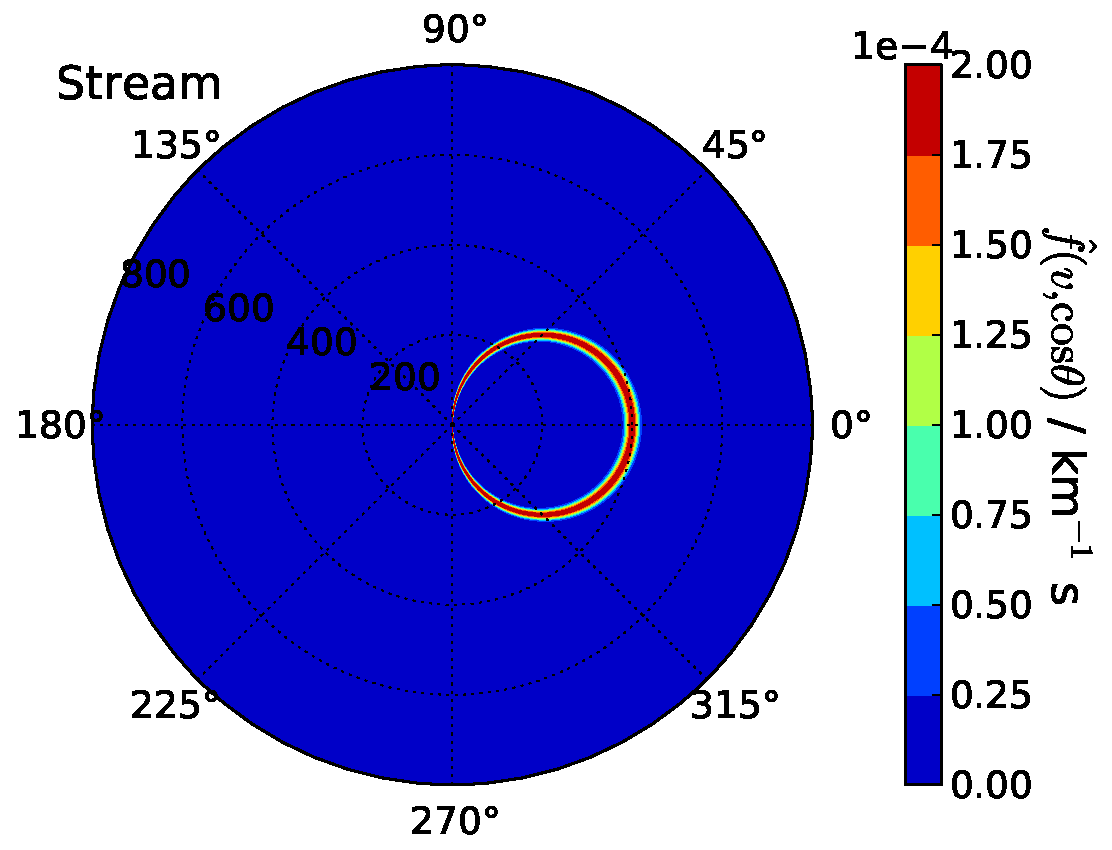
\includegraphics[width=0.75\textwidth]{Directional/STREAMRadonpolar.pdf}

\caption[Radon transform examples]{Radon transform $\hat{f}(\vmin, \cos\theta)$ of the SHM (top), SHM with a dark disk contribution (middle) and stream (bottom) distribution functions. We have integrated over the $\phi$ angle. In each case $\mathbf{v}_\textrm{lag}$ is aligned along $\theta = 0$. Note the different scale in each plot.}
  \label{fig:directional:Radon}
\end{figure}


\section{Directional experiments}
\label{sec:directional:experiments}

Directional experiments are still in the prototype stage. A number of experiments use time projection chamber (TPC) technology to achieve directional sensitivity. These include DRIFT \cite{Daw:2011,Daw:2012}, NEWAGE \cite{Miuchi:2010,Miuchi:2012}, MIMAC \cite{Riffard:2013, Santos:2013}, DMTPC \cite{Monroe:2012,Battat:2013} and D3 \cite{Vahsen:2012}. These detectors are less than 1 $\textrm{m}^3$ in size, with hopes for a scale up to larger experiments (possibly up to ton-scale) in the future.

In order to have directional sensitivity, a detector must image the tracks produced by the recoiling nucleus in the detector. The typical range of a WIMP-nucleus recoil is only $\sim$100 nm, however, which makes track reconstruction difficult. The above directional experiments therefore operate in the low pressure gas phase (around 0.05 atm \cite{Daw:2012}) in order to maximise the distance travelled by a recoiling nucleus. The detector is filled with a target gas (such as $CF_4$ in the case of the DRIFT experiment) which provides sensitivity predominantly to spin-dependent interactions. Nuclear recoils in the detector ionize the target gas. The freed electrons are drifted under an electric field to an anode at one face of the detector where the charge is collected. An electron transport gas ($CS_2$ in the DRIFT experiment) may also be added, which attracts the free electrons forming ions which are then collected.

The energy of the recoil can be recovered from the total amount of ionisation in the event. The three dimensional track (which is only a few mm long) can be reconstructed from the distribution of charge detected at the anode, with information about the z-direction obtained from the timing of the charges arriving at the anode. This method allows an angular resolution of 20$\,^{\circ}$-80$\,^{\circ}$ using current prototypes \cite{Billard:2012}, with higher resolution at higher recoil energies. However, the sense of the recoil is much more difficult to determine, requiring sensitivity to tiny asymmetries between the start and end of the track. While sense discrimination has previously been demonstrated \cite{Burgos:2008}, it cannot be achieved with 100\% efficiency. Even for high energy (100 keV) recoils, studies suggest that only partial sense recognition may be possible (with only a 65\% probability of correctly determining the sense) \cite{Billard:2012}. Without sense discrimination the anisotropy of the WIMP signal is reduced and roughly 3 times more events are required to establish the directionality of the signal and distinguish from an anisotropic background \cite{Morgan:2005,Green:2008}.

%\note{Background - Radon progeny; fiducialisation; thresholds}

A number of other directional technologies have also been suggested. Nuclear emulsion experiments use as a target silver halide crystals suspended in gelatin \cite{Naka:2012}. The emulsion required must be composed of very fine grains in order to image dark matter recoil tracks smaller than 1 $\mu \textrm{m}$. However, angular resolutions below 20$\,^{\circ}$ may be achievable. DNA based experiments \cite{Drukier:2012} have also been proposed which may be able to achieve directional sensitivity. The collaborations running the main TPC-based experiments have proposed a joint project to construct a ton-scale `CYGNUS' detector \cite{Ahlen:2009} in the future.


\section{Reconstructing the velocity distribution}

With promising developments in directional detector technology, it is interesting to ask what information about the velocity distribution we could, in principle, extract from a directional signal. Alves, Hendri and Wacker \cite{Alves:2012} investigated the possibility of describing $f(\textbf{v})$ in terms of a series of special functions of integrals of motion (energy and angular momentum). These can then be fit to data, with around 1000 events required to distinguish between the SHM and a Via Lactea II distribution function \cite{Kuhlen:2008}. However, the special, separable form of the velocity distribution requires that the dark matter halo is in equilibrium. Moreover, this method requires prior knowledge of the DM mass (for example from earlier non-directional detectors or from collider experiments).

A more general parametrisation for the velocity distribution was recently proposed by Lee \cite{Lee:2014}. In this approach, the velocity distribution is decomposed into products of Fourier-Bessel functions and spherical harmonics. This is completely general and does not require that the halo is completely virialised. Lee also gives an analytic expression for the Radon transform of the Fourier-Bessel basis, making this approach computationally efficient. However, this basis does not guarantee that the resulting $f(\textbf{v})$ is everywhere positive and therefore not all combinations of coefficients correspond to physical distribution functions. %\note{Might be a good idea after a large number of events have been found...}

In fact, any decomposition in terms of spherical harmonics leads to this problem, because the spherical harmonic basis functions can have negative values. It is unclear how this issue will affect parameter reconstruction. Without some criteria which determines which coefficients of the spherical harmonics lead to strictly positive distribution functions, it may be necessary to numerically test each parametrised distribution function for negative values. However, for a real function of three parameters $f(\textbf{v}) = f(v_x, v_y, v_z)$ this would require a very large number of evaluations, which may not be computationally feasible. In addition, it is not clear how this property would affect an exploration of the parameter space using, for example, Markov Chain Monte Carlo or Nested Sampling (see Appendix~\ref{ch:ParamRecon}). Physical distribution functions may occupy only a small fraction of the total space of parameters or may be distributed over a large number of irregular regions in the parameter space, making sampling from them difficult.

In order to fit to data, it is necessary to decompose $f(\textbf{v})$ into a series of angular components $A^i$:
\begin{equation}
f(\textbf{v}) = f^1(v) A^1(\theta',\phi') + f^2(v) A^2(\theta',\phi') +f^3(v) A^3(\theta',\phi') +...\,.
\end{equation}
We then truncate the series at some order, leaving only a finite number of 1-dimensional functions $f^i(v)$ which are unknown. This reduces the problem of attempting to fit a function of the 3-dimensional variable $\textbf{v}$ to the problem of parametrising a series of 1-dimensional functions, which is much more tractable. Of course, we should be careful that this truncation preserves enough angular information to still provide a good approximation to $f(\textbf{v})$. However, as more data becomes available, we can add more terms to the series to capture more angular features in the distribution.

As we have discussed, the spherical harmonic basis may not be an appropriate choice for this decomposition. In the next section, I will present an alternative decomposition which can guarantee that the velocity distribution is everywhere positive and therefore represents a promising and general method for extracting information from directional experiments.

%\todo{Point out that this is harder when you have a full 3-D function...?}

\begin{comment}

\subsection{Invertibility of the Radon transform}

\todo{Make sure to check and improve the terminology - especially `null functions'}

It has been shown that for distributions \(f(\textbf{v})\) which are rapidly decreasing at infinity \cite{Helgason:1999} or which are compactly supported \cite{Quinto:1983}, the Radon Transform is one-to-one and is therefore exactly invertible. This inversion is typically unstable (that is, the reconstructions are very sensitive to noise in the signal) and ill-posed (as not all functions are valid Radon Transforms). However, assuming that \(\hat{f}\) is a valid Radon Transform and that we have full knowledge of it, we can reconstruct $f(\textbf{v})$ exactly.

However, due to finite energy thresholds, we do not have access to the low-speed region of $\hat{f}(v_\textrm{min}, \hat{q})$. We must therefore consider the related Exterior Radon Transform \(\mathcal{R}_E\). Only using values of the Radon Transform for \(v_{\textrm{min}} > v_a\), is it possible to reconstruct $f(\textbf{v})$ for $v > v_a$? If \(f\) is rapidly decreasing at infinity, this transform is still one-to-one, as in the complete case. However, if \(f\) decays as an inverse power of \(v\) (i.e.\ \(f \sim v^{-k}\) as \(v\rightarrow \infty\)) the Exterior Transform is no longer one-to-one \cite{Shepp:1978}. \todo{Define null space...} In this case, the null space in 3 dimensions is non-trivial \cite{Quinto:1982}, consisting of functions of the form:

\begin{equation}
\label{eq:null}
f_N(\textbf{v}) = \frac{\alpha}{v^{3+k}} Y_{lm}(\hat{\textbf{v}}),
\end{equation}
where \(\alpha\) is some constant, \(Y_{lm}\) is a spherical harmonic, \(0 \leq k < l\) and \(l-k\) is even. This means that there are no null functions for \(l = 0\) or \(l = 1\). It can be shown by explicit calculation that such functions have a Radon Transform of zero for all \(v_\textrm{min} > 0\).

In the case of direct detection, the point at \(v = v_\textrm{min} = 0\) corresponds to DM particles at rest with respect to the detector, which can impart no recoil energy and are therefore undetectable. For directional detection then, even for infinitesimally small threshold energies, we must consider the Exterior Radon Transform.

This means that for a given Radon transform, adding any combination of functions of the form $f_N(\textbf{v})$ to $f(\textbf{v})$ leads to the same Radon transform. However, we note that the spherical harmonics with \(l > 0\) can take negative values. However, at large values of \(v\), \(f_\textrm{SHM}\) decays exponentially. By contrast, \(f_N\) decays as a power of \(v\), meaning at some (potentially large) value of \(v\) the magnitude of the null function will exceed that of \(f(\textbf{v})\) leading to a negative distribution function. A more general distribution function will have a natural cut-off (say at the galactic escape speed) and will certainly decay rapidly to zero for high values of \(v\). As a result, we can neglect the impact of null functions on reconstructions.

Thus, as long as we choose basis functions which are everywhere positive and therefore physically valid, we ensure that the Radon transform is invertible. This means that no information is lost in reconstructing $f(\textbf{v})$ and also that there are no unphysical degeneracies present in the parametrisation we have chosen.

\todo{NB: Make it very clear that if we choose a parametrisation which can be somewhere negative (even if it's a high energies where these things don't matter because its above threshold and only a small effect), it can lead to problems of non-invertibility and introduce unphysical degeneracies in the parametrisation. Therefore it is very important to make sure that $f(\textbf{v})$ is everywhere positive. I should include some plots of the null functions and of truncated null functions (added to $f(\textbf{v})$) to indicate what can go wrong - and how bad things can be. Also, talk about truncated null functions and check that if we ensure positive-definiteness then truncated null functions shouldn't cause a problem... Double-check to see if truncated null functions (truncated at the same place as the full distribution function) are still null (they shouldn't be, don't just look along one direction, but all... IT DEFINITELY IS NOT NULL, SO THAT'S FINE...)}

\note{Also say that I don't think that this has previously been discussed...}

\end{comment}

\section{Discretising the velocity distribution}
\label{sec:directional:discretising}

In order to ensure that the velocity distribution is everywhere positive, we propose that the velocity distribution be discretised into $N$ angular components:

\begin{equation}
f(\textbf{v}) = f(v, \cos\theta', \phi') =
\begin{cases}
f^1(v) & \textrm{ for } \theta' \in \left[ 0, \pi/N\right]\,, \\
f^2(v) & \textrm{ for } \theta' \in \left[ \pi/N, 2\pi/N\right]\,, \\
 & \vdots\\
f^k(v) & \textrm{ for } \theta' \in \left[ (k-1)\pi/N, k\pi/N\right]\,, \\
 & \vdots\\
f^N(v) & \textrm{ for } \theta' \in \left[ (N-1)\pi/N, \pi\right]\,. \\
\end{cases}
\end{equation}
Over each bin in $\theta'$, $f(\textbf{v})$ has no angular dependence and depends only on a single function of the WIMP speed. We consider for simplicity only a discretisation in $\cos\theta'$, though this can be extended to an additional discretisation in $\phi'$ if required.


We show in Fig.~\ref{fig:directional:Discrete} an example of this discretised velocity distribution. We show the full SHM velocity distribution (top), as well as the $N=2$ (middle) and $N=3$ (bottom) discretised approximations. These approximations are obtained by averaging the full velocity distribution over each bin in $\theta'$.

\begin{figure}[pht!]
  \centering
  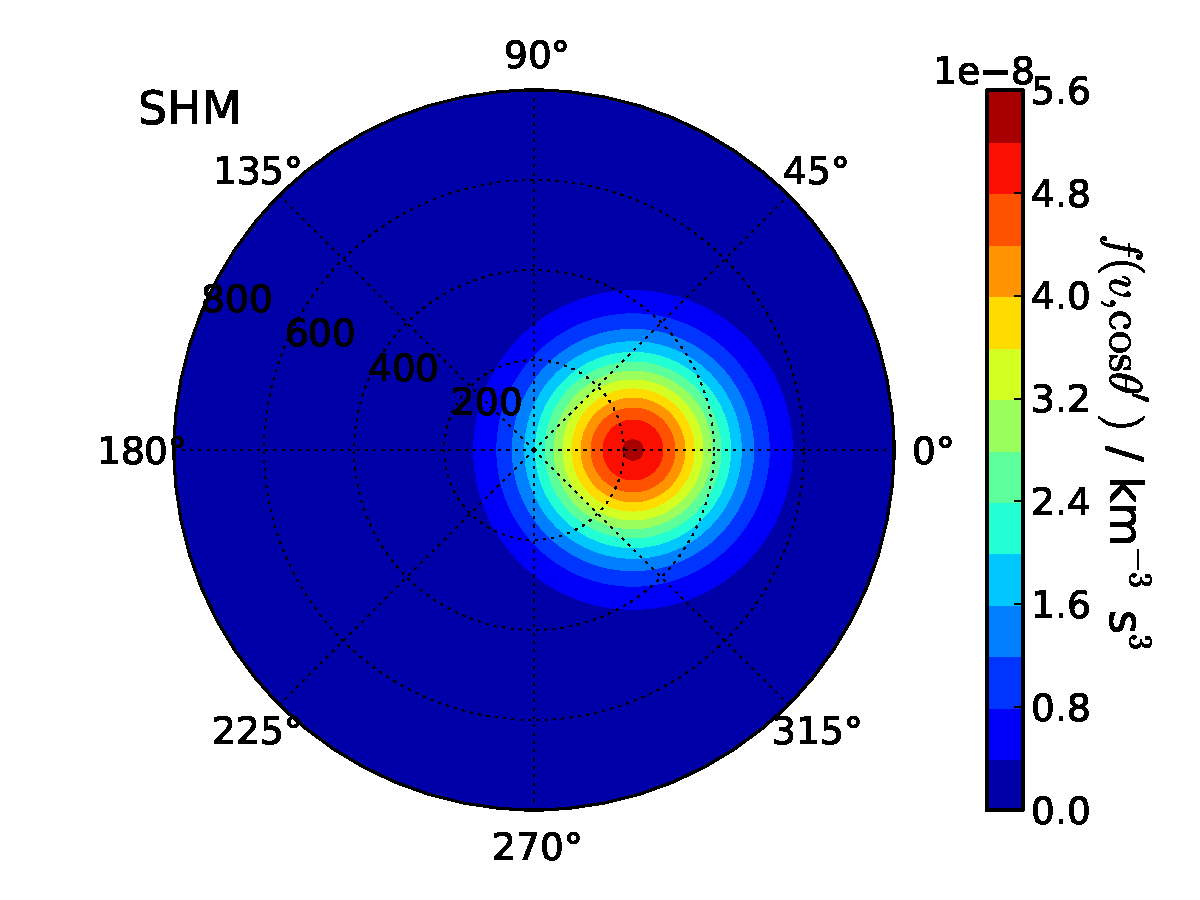
\includegraphics[width=0.75\textwidth]{Directional/SHMpolar.pdf}

  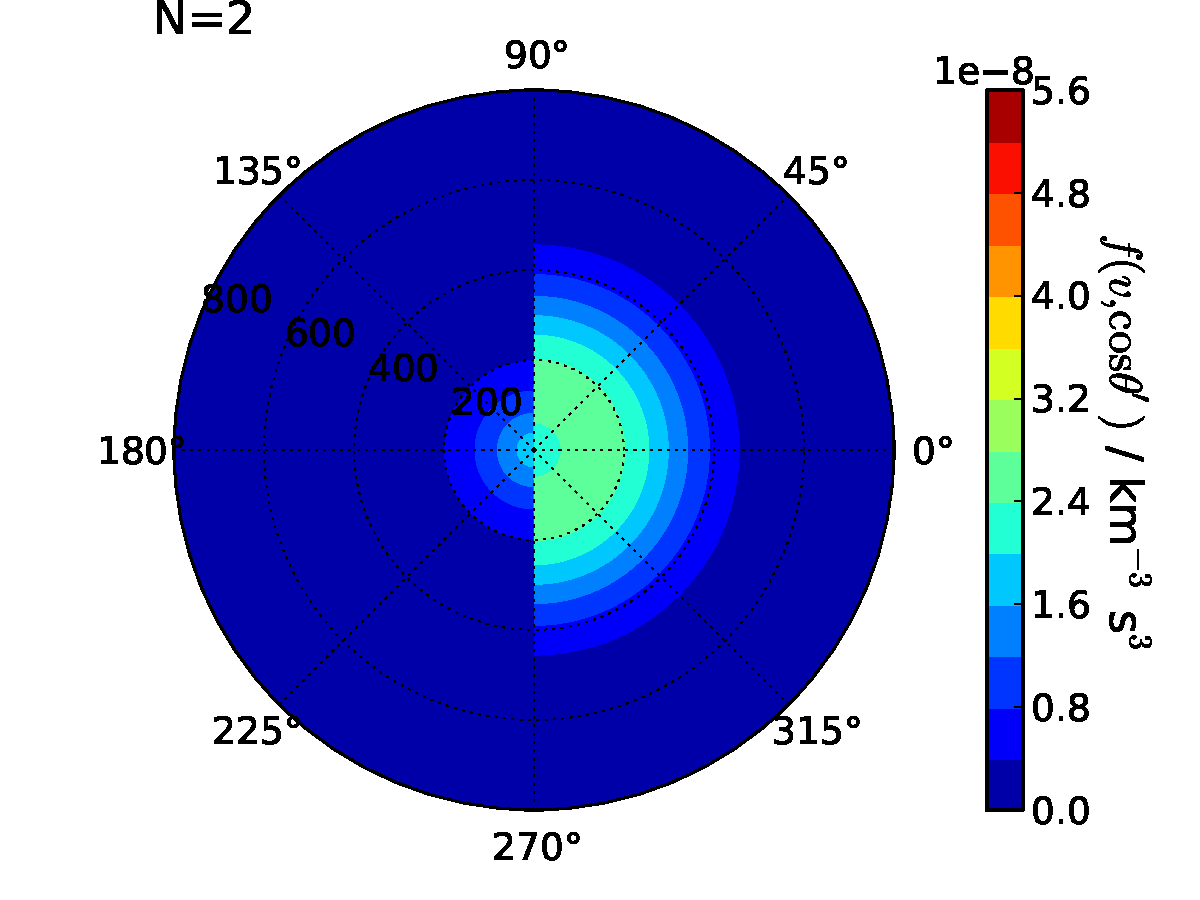
\includegraphics[width=0.75\textwidth]{Directional/SHMpolarN2.pdf}
  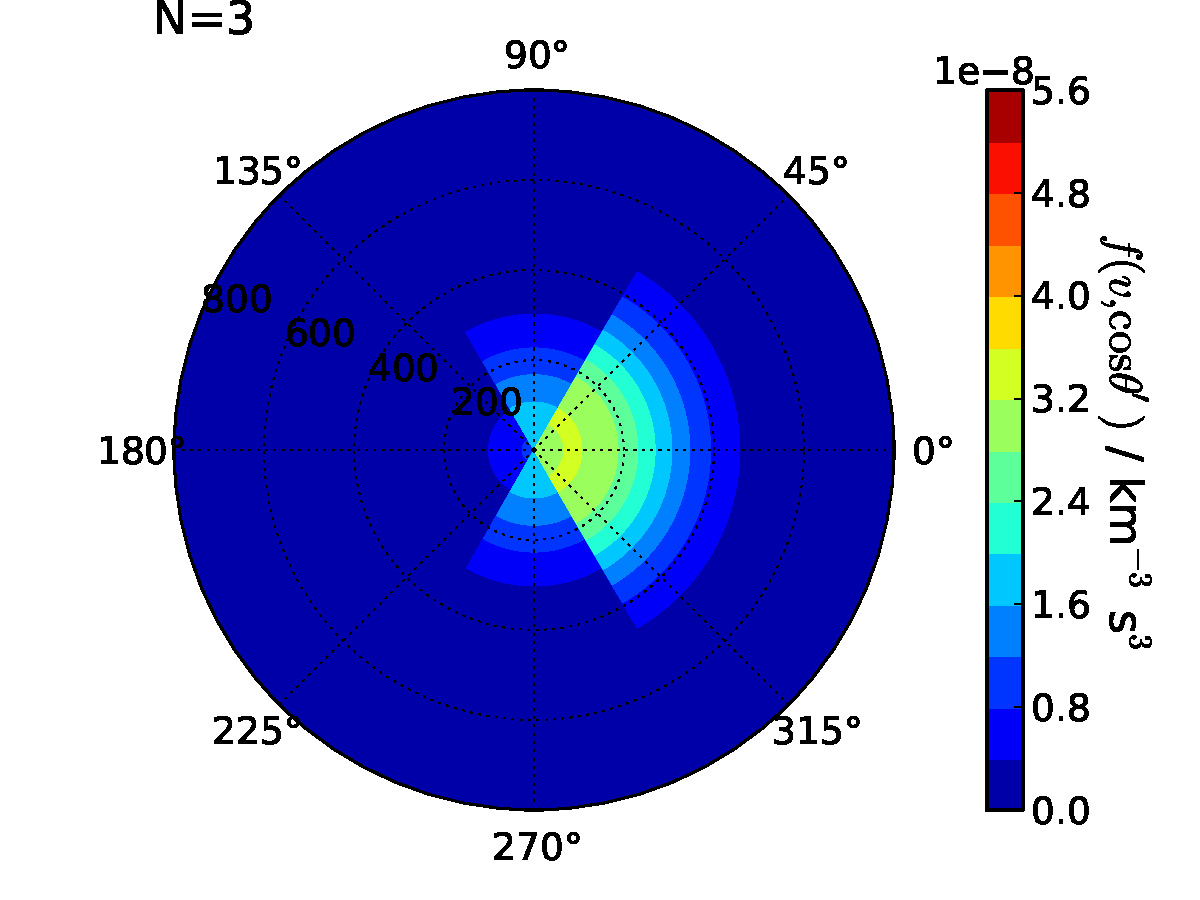
\includegraphics[width=0.75\textwidth]{Directional/SHMpolarN3.pdf}

\caption[Examples of discretised velocity distributions]{The SHM velocity distribution (top) as well as $N=2$ (middle) and $N=3$ (bottom) discretised approximations. In each case, we have integrated over the $\phi'$ direction and only show $f(v, \cos\theta')$. The vector $\textbf{v}_\textrm{lag}$ is aligned along $\theta' = 0$. The same colour scale is used in each plot.}
  \label{fig:directional:Discrete}
\end{figure}

The motivation for this description is that the simplest signal (beyond an isotropic $N=1$ signal) which can be observed with a directional detector is an asymmetry between the event rates in, say, the forward and backward directions. Shortly after the confirmation of a dark matter signal at a directional detector, the number of events may still be quite small (for example, the roughly 10 events required to distinguish from an isotropic background). In this small statistics scenario, constraining a large number of free functions is not feasible. However, if we discretise $f(\textbf{v})$ into $N=2$ angular components, it should be possible to extract some meaningful directional information with only a small number of events. With larger numbers of events, $N$ can be increased to allow more directional information to be extracted.

Because angular information is being lost from the velocity distribution, the full Radon transform of this discretised distribution is unlikely to provide a good fit to the data on an event by event basis. Instead, we should consider integrated Radon transforms of the form:

\begin{equation}
\hat{f}^k(v_\textrm{min}) = \int_{\phi = 0}^{2\pi} \int_{(k-1)\pi/N}^{k\pi/N} \hat{f}(v_\textrm{min}, \hat{\textbf{q}})\, \mathrm{d}\cos\theta\mathrm{d}\phi,
\end{equation}
 where $\hat{\textbf{q}} = (\cos\theta, \phi)$. Thus, we will be using a discretised version of the Radon transform (or equivalently, the event rate and, ultimately, data) in order to constrain the functional form of the discretised velocity distribution. While binning the data in this way results in a loss of angular information, it should reduce the error which is introduced by using a binned approximation to the velocity distribution. This in turn allows us to parametrise the $v$-dependence of each angular bin and mitigate uncertainties in the velocity distribution.

What form should be used for the free functions $f^k(v)$? This discretisation scheme does not depend on choosing a particular form for the $v$-dependence of the velocity distribution. We can therefore choose any parametrisation for $f^k(v)$ - such as the polynomial parametrisation described in Chapter~\ref{ch:Poly} - as long as it is everywhere positive and we are convinced that it introduces no bias into the fitting procedure. The question we will now address is what errors are introduced by this angular discretisation. We will now demonstrate for the cases of $N=1, 2, 3$ how the corresponding Radon transform is calculated and how it compares to the true Radon transform for some benchmark cases.


%\todo{Talk somewhere about tomography...}

\subsection{$N=1$ discretisation}

The $N=1$ case corresponds to the assumption that $f(\textbf{v})$ is isotropic. That is, we could consider setting $f(\textbf{v})$ equal to its angular average:

\begin{equation}
\label{eq:directional:isotropic}
f(\textbf{v}) = \bar{f}(v) \equiv \frac{1}{4\pi} \int f(\textbf{v}) \, \mathbf{d}\Omega_v\,.
\end{equation}
The Radon transform then reduces to
\begin{equation}
\label{eq:directional:radonN1}
\hat{f}\left(v_\textrm{min},\hat{\textbf{q}}\right) = \int \delta\left(v_\textrm{min} - \textbf{v}\cdot\hat{\textbf{q}}\right) \bar{f}(v) \,\textrm{d}^3\textbf{v}\,.
\end{equation}

We can rewrite the delta function as

\begin{equation}
\delta\left(v_\textrm{min} - \textbf{v}\cdot\hat{\textbf{q}}\right) = \frac{1}{v}\delta(v_\textrm{min}/v - \hat{\textbf{v}}\cdot\hat{\textbf{q}})\,,
\end{equation}
which means that Eq.~\ref{eq:directional:radonN1} becomes

\begin{equation}
\hat{f}\left(v_\textrm{min},\hat{\textbf{q}}\right) = \int_{v=0}^\infty \frac{v^2\bar{f}(v)}{v} \oint \delta\left(v_\textrm{min}/v - \hat{\textbf{v}}\cdot\hat{\textbf{q}}\right)  \, \mathrm{d}\Omega_v\mathrm{d}v\,.
\end{equation}
The angular integral evaluates to unity as long as $v_\textrm{min}/v = \hat{\textbf{v}}\cdot\hat{\textbf{q}}$ for some value of $\hat{\textbf{v}}$ in the domain of integration. Because we integrate over all directions $\hat{\textbf{v}}$, this is guaranteed to be satisfied for some value, as long as $v > v_\textrm{min}$ (because $\hat{\textbf{v}}\cdot\hat{\textbf{q}}$ cannot exceed 1). Thus,

\begin{equation}
\oint \delta\left(v_\textrm{min}/v - \hat{\textbf{v}}\cdot\hat{\textbf{q}}\right)  \, \mathrm{d}\Omega_v = \Theta(v - v_\textrm{min})\,,
\end{equation}
and
\begin{equation}
\hat{f}\left(v_\textrm{min},\hat{\textbf{q}}\right) = \int_{v=v_\textrm{min}}^\infty \frac{v^2\bar{f}(v)}{v} \mathrm{d}v\,.
\end{equation}

Finally, to obtain the directionally averaged Radon transform $\hat{f}(v_\textrm{min})$, we integrate over all directions $\qhat$. As the Radon transform is isotropic in this case, this gives a contribution of $4\pi$. Replacing the expression for $\bar{f}(v)$ from Eq.~\ref{eq:directional:isotropic}, we therefore obtain

\begin{equation}
\hat{f}\left(v_\textrm{min}\right) = \int_{v=v_\textrm{min}}^\infty \frac{f(\textbf{v})}{v} \mathrm{d}^3\textbf{v}\,.
\end{equation}

This matches the expression for the total non-directional scattering rate. We therefore see that in the $N=1$ case, the angular-discretised `approximation' is in fact exact and leads to the correct angular-averaged Radon transform.


\subsection{$N=2$ discretisation}


For the $N=2$ case, we are considering a forward-backward asymmetry in the velocity distribution:

\begin{equation}
\label{eq:directional:N2}
f(\mathbf{v}) =
\begin{cases}
f^1(v) & \textrm{for } \theta' \in [0, \pi/2]\,, \\
f^2(v) & \textrm{for } \theta' \in [\pi/2, \pi]\,.
\end{cases}
\end{equation}

From these, we wish to obtain the integrated Radon transforms for the forward and backward directions. Specifically:

\begin{align}
\hat{f}^1(\vmin) &= \int_{0}^1 \hat{f}(\vmin,\cos\theta) \, \mathrm{d}\cos\theta\,, \\
\hat{f}^2(\vmin) &= \int_{-1}^0 \hat{f}(\vmin, \cos\theta) \, \mathrm{d}\cos\theta \,.
\end{align}
Full details of the calculation are given in Appendix~\ref{ch:RadonCalc}. However, the result takes the relatively straightforward form:

\begin{align}
\label{eq:directional:N2result}
\hat{f}^1 &= 4\pi\int_{\vmin}^{\infty} v \left\{ \pi f^1(v) + \atan\left(\frac{\sqrt{1-\beta^2}}{\beta}\right)\left[f^2(v) - f^1(v)\right] \right\} \, \mathrm{d}v \,,\\
\hat{f}^2 &= 4\pi\int_{\vmin}^{\infty} v \left\{ \pi f^2(v) + \atan\left(\frac{\sqrt{1-\beta^2}}{\beta}\right)\left[f^1(v) - f^2(v)\right] \right\} \, \mathrm{d}v\,,
\end{align}
where $\beta = \vmin/v$. We have also checked using Monte Carlo calculations that these are the correct forms of the forward and backward integrated Radon transforms in the case of a discretised velocity distribution.


We now wish to compare these approximate Radon transforms with the Radon transforms obtained from the full (non-discretised) velocity distribution. To do this, we select a benchmark velocity distribution (such as the SHM) and calculate the $f^{1,2}$ of Eq.~\ref{eq:directional:N2} by averaging over $\cos\theta'$ in the forward and backward directions as in Fig.~\ref{fig:directional:Discrete}. We then insert these into Eq.~\ref{eq:directional:N2result} to obtain the forward and backward Radon transforms. We refer to these as the \textit{approximate} forward and backward Radon transforms. For comparison, we use the full Radon transform of Eq.~\ref{eq:directional:SHM} to obtain the \textit{exact} forward and backward Radon transforms by integrating over $\cos\theta$.


The results of this comparison for an SHM model with $v_\textrm{lag} = 220 \kms$ and $\sigma_v = 156 \kms$ are shown in Fig.~\ref{fig:directional:radonN2_SHM}. While the general features are reproduced, there are some discrepancies. In particular, the forward Radon transform obtained using the approximate method is roughly 80\% of the correct result, while the backward Radon transform is up to 100\% larger using the approximate method (though only when the absolute value becomes small). The reason for this is clear from Fig.~\ref{fig:directional:Discrete}, which shows that the discretised velocity distribution has a greater fraction of WIMPs with velocities at right angles to the forward direction ($\theta' = 0$). Thus, the discretised velocity distribution has a greater chance of producing scatters in the backward direction. Overall, the discretised distribution is less focused in the forward direction, resulting in a reduced asymmetry between the forward and backward scattering rates.

\begin{figure}[ht!]

  \centering
  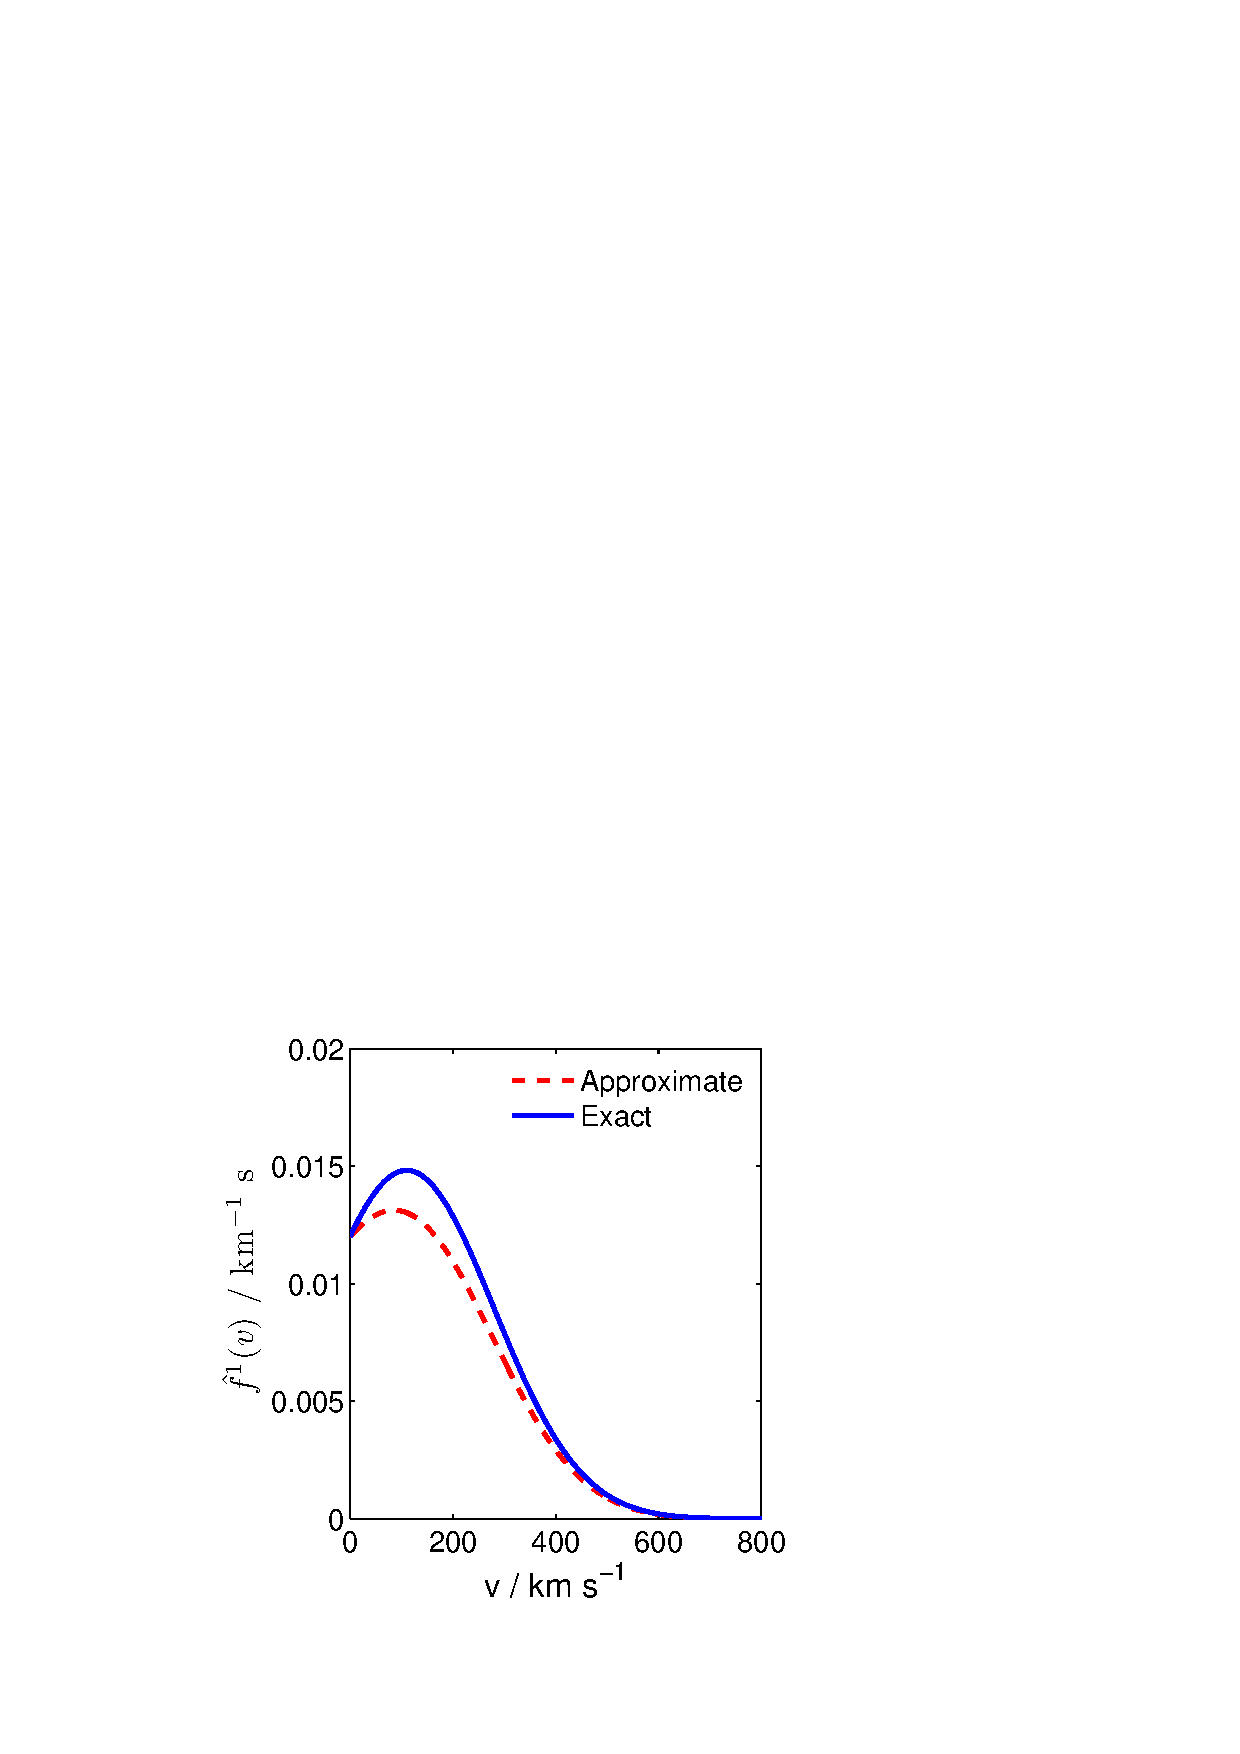
\includegraphics[trim={3.5cm 2cm 7.5cm 17cm},clip,width=0.49\textwidth]{Directional/SHM_N2_1.pdf}
  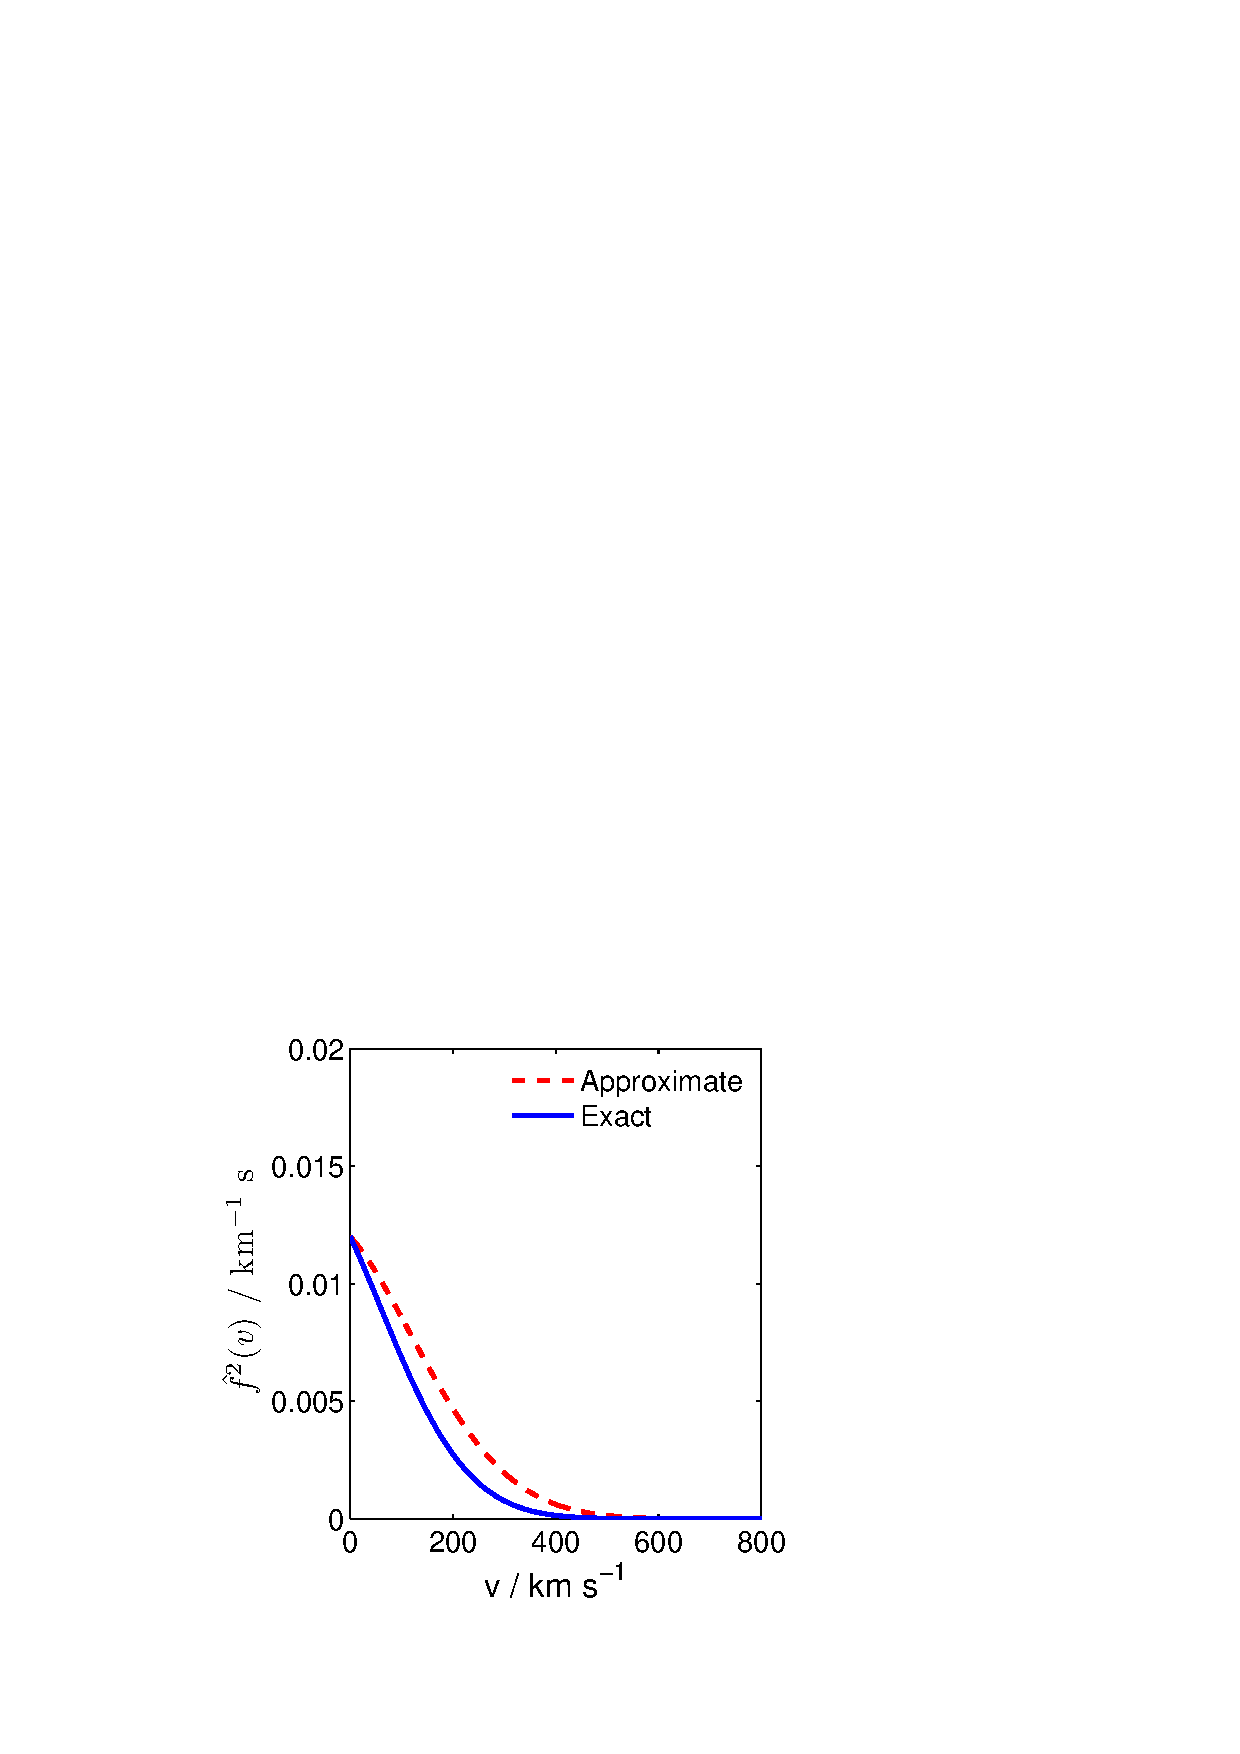
\includegraphics[trim={3.5cm 2cm 7.5cm 17cm},clip,width=0.49\textwidth]{Directional/SHM_N2_2.pdf}

\caption[Exact and approximate integrated Radon transforms for $N=2$ components in the SHM]{Exact and approximate forward and backward Radon transforms, $\hat{f}^1$ and $\hat{f}^2$, for the SHM. The approximate Radon transforms are obtained by discretising the full velocity distribution into N = 2 angular bins. The vector $\textbf{v}_\textrm{lag}$ is aligned along $\theta' = 0$.}
\label{fig:directional:radonN2_SHM}
\end{figure}

We show in Fig.~\ref{fig:directional:radonN2_STREAM} the forward and backward Radon transforms for a stream distribution function, with $v_\textrm{lag} = 400 \kms$ and $\sigma_v = 20 \kms$. The discrepancy between the approximate and exact results is significantly worse in this case. This is because the stream is highly directional and a simple $N=2$ discretisation of the velocity distribution is not sufficient to capture the angular features of the stream

\begin{figure}[ht!]

  \centering
  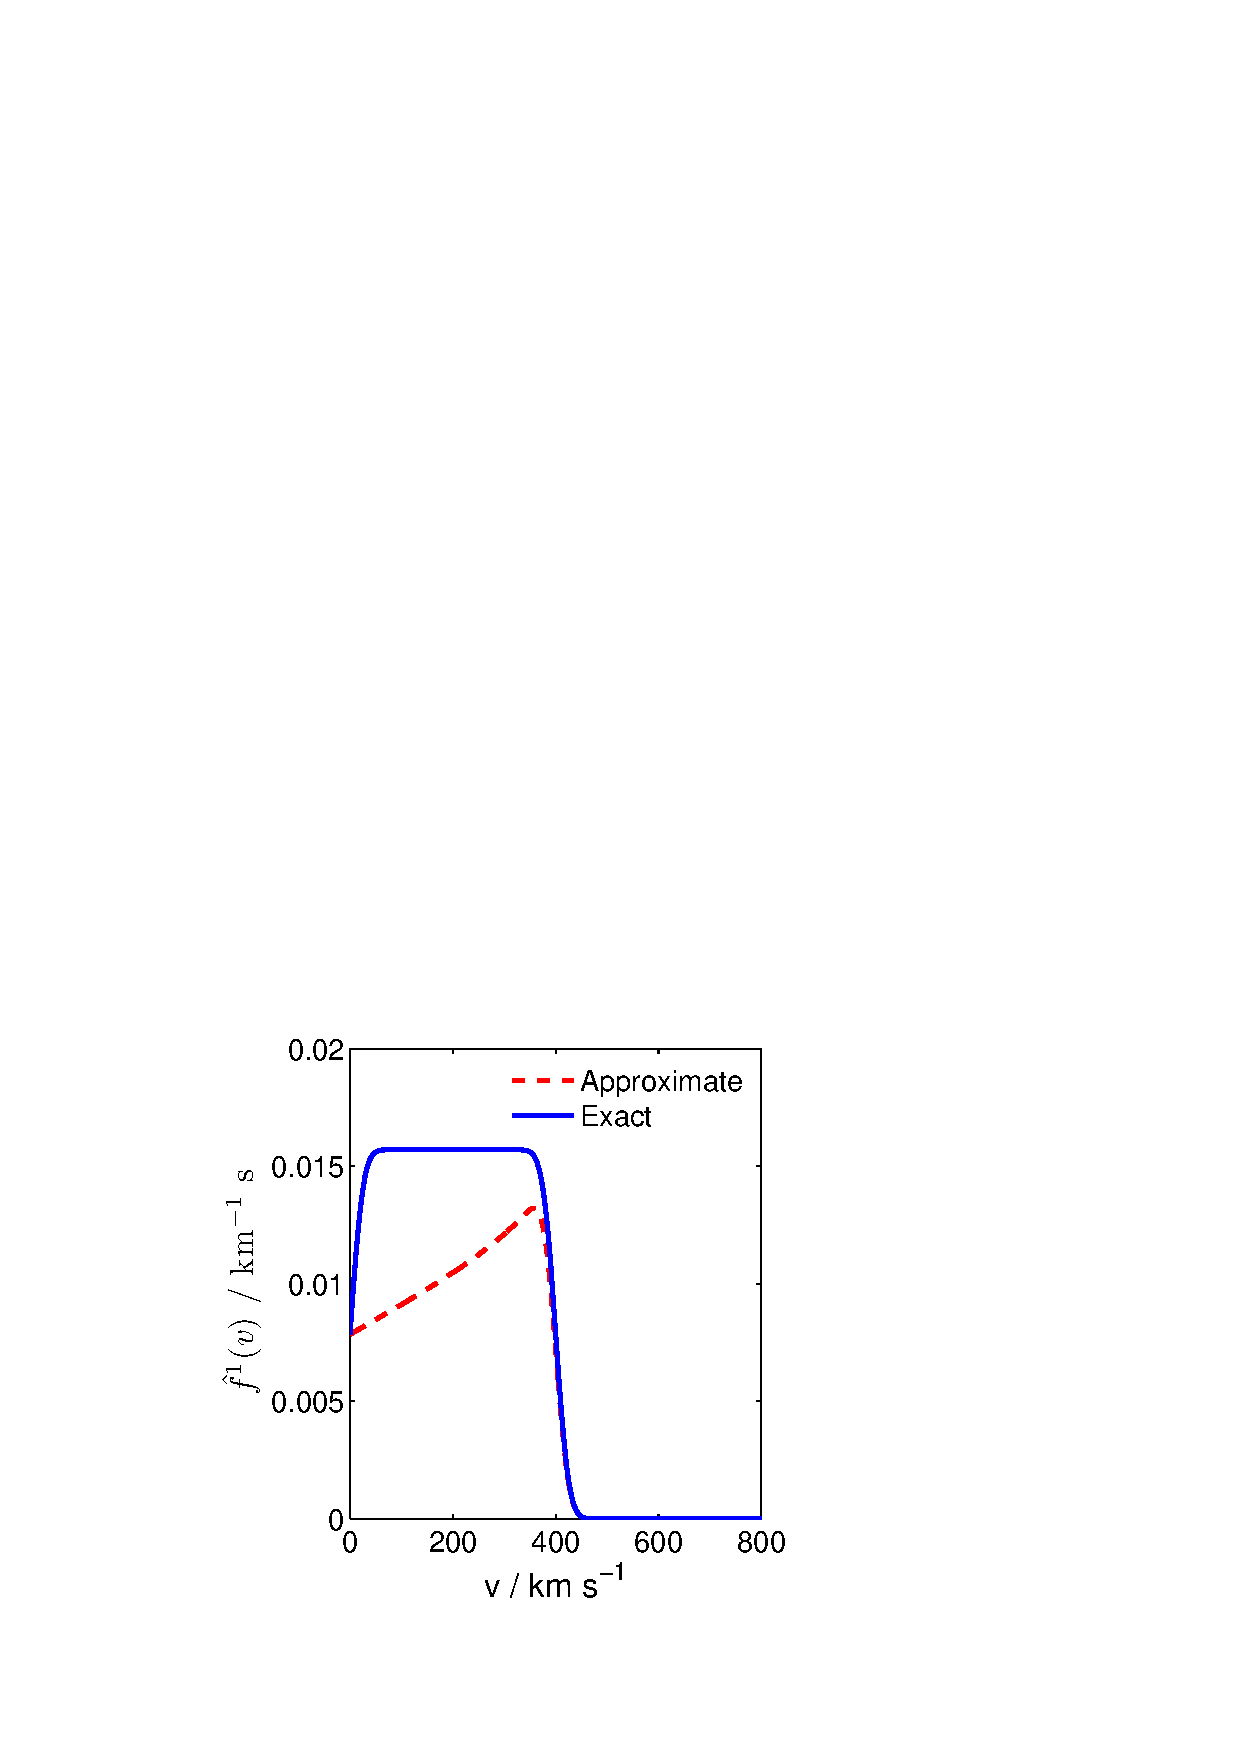
\includegraphics[trim={3.5cm 2cm 7.5cm 17cm},clip,width=0.49\textwidth]{Directional/STREAM_N2_1.pdf}
  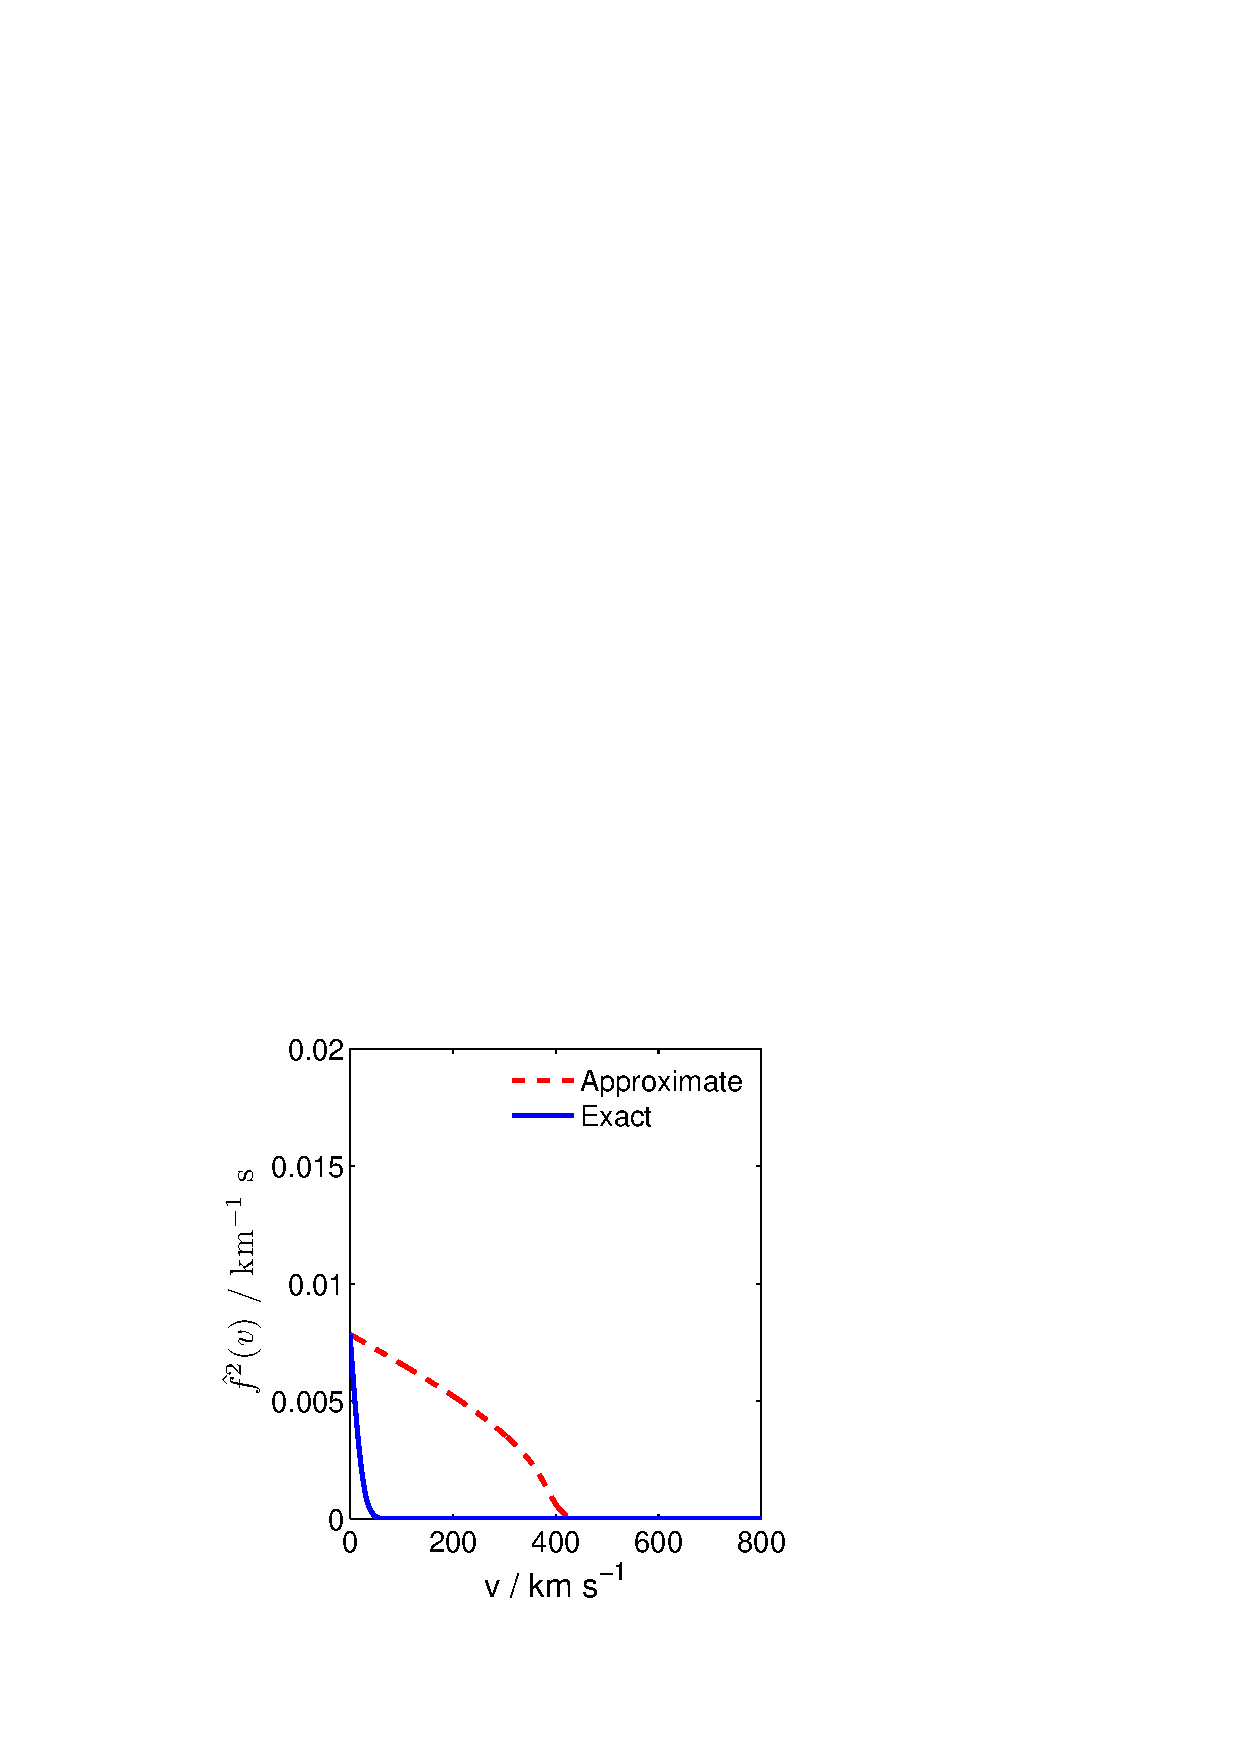
\includegraphics[trim={3.5cm 2cm 7.5cm 17cm},clip,width=0.49\textwidth]{Directional/STREAM_N2_2.pdf}

\caption[Exact and approximate integrated Radon transforms for $N=2$ components for a stream distribution function]{As Fig.~\ref{fig:directional:radonN2_SHM}, but for a stream distribution with $v_\textrm{lag} = 400 \kms$ and $\sigma_v = 20 \kms$.}
\label{fig:directional:radonN2_STREAM}
\end{figure}



%These discrepancies between the true and approximate recoil spectra may prove problematic when this method is employed in parameter estimation and the reconstruction of $f(\textbf{v})$. However, these discrepancies should be redued when the finite angular resolution of detectors is taken into account. \todo{Mention finite angular resolution...Do some plots...}

%\todo{Consider a more radical distribution - such as a stream and show that it doesn't work so well...}

\subsection{$N=3$ discretisation}

Given the discrepancies in the $N=2$ case, we will now consider the $N=3$ discretisation, which should improve the fit between the true and approximate transforms. In addition, $N=3$ will allow us to employ this methodology to the case where sense discrimination of recoils is not possible. Without sense discrimination, the forward and backward directions cannot be distinguished and the $N=2$ discretisation provides no directional sensitivity. As we shall see shortly, directional sensitivity is possible in the $N=3$ case.

We write the velocity distribution in discretised form as

\begin{equation}
\label{eq:directional:N3}
f(\mathbf{v}) =
\begin{cases}
f^1(v) & \textrm{for } \theta' \in [0, \pi/3] \\
f^2(v) & \textrm{for } \theta' \in [\pi/3, 2\pi/3] \\
f^3(v) & \textrm{for } \theta' \in [2\pi/3, \pi]\,.
\end{cases}
\end{equation}

If we interpret this discretisation as an averaging of the underlying velocity distribution, as before, we obtain the distribution in the bottom panel of Fig.~\ref{fig:directional:Discrete} for the SHM. Following the same procedure as for the $N=2$ case, we can obtain the corresponding forward, backward and transverse integrated Radon transforms. The exact form of these is complicated (and not particularly instructive), so we do not include it in full here. However, as in the $N=2$ case, we can test these approximate transforms against the exact forms.

The results for the SHM are shown in Fig.~\ref{fig:directional:radonN3_SHM}. Compared to the $N=2$ case, the Radon transforms are reproduced much more closely, with a discrepancy of at most 15\% between the true and approximate distributions. As can be seen in the bottom panel of Fig.~\ref{fig:directional:Discrete}, the $N=3$ discretised velocity distribution is more focused in the forward direction and fewer particles have velocities perpendicular $\textbf{v}_\textrm{lag}$. In Fig.~\ref{fig:directional:radonN3_STREAM}, we show the corresponding results for the stream distribution. These show a slight improvement over the $N=2$ case (particularly in the backward rate). However, there are still significant differences between the exact and approximate Radon transforms.

\begin{figure}[ht!]

  \centering
  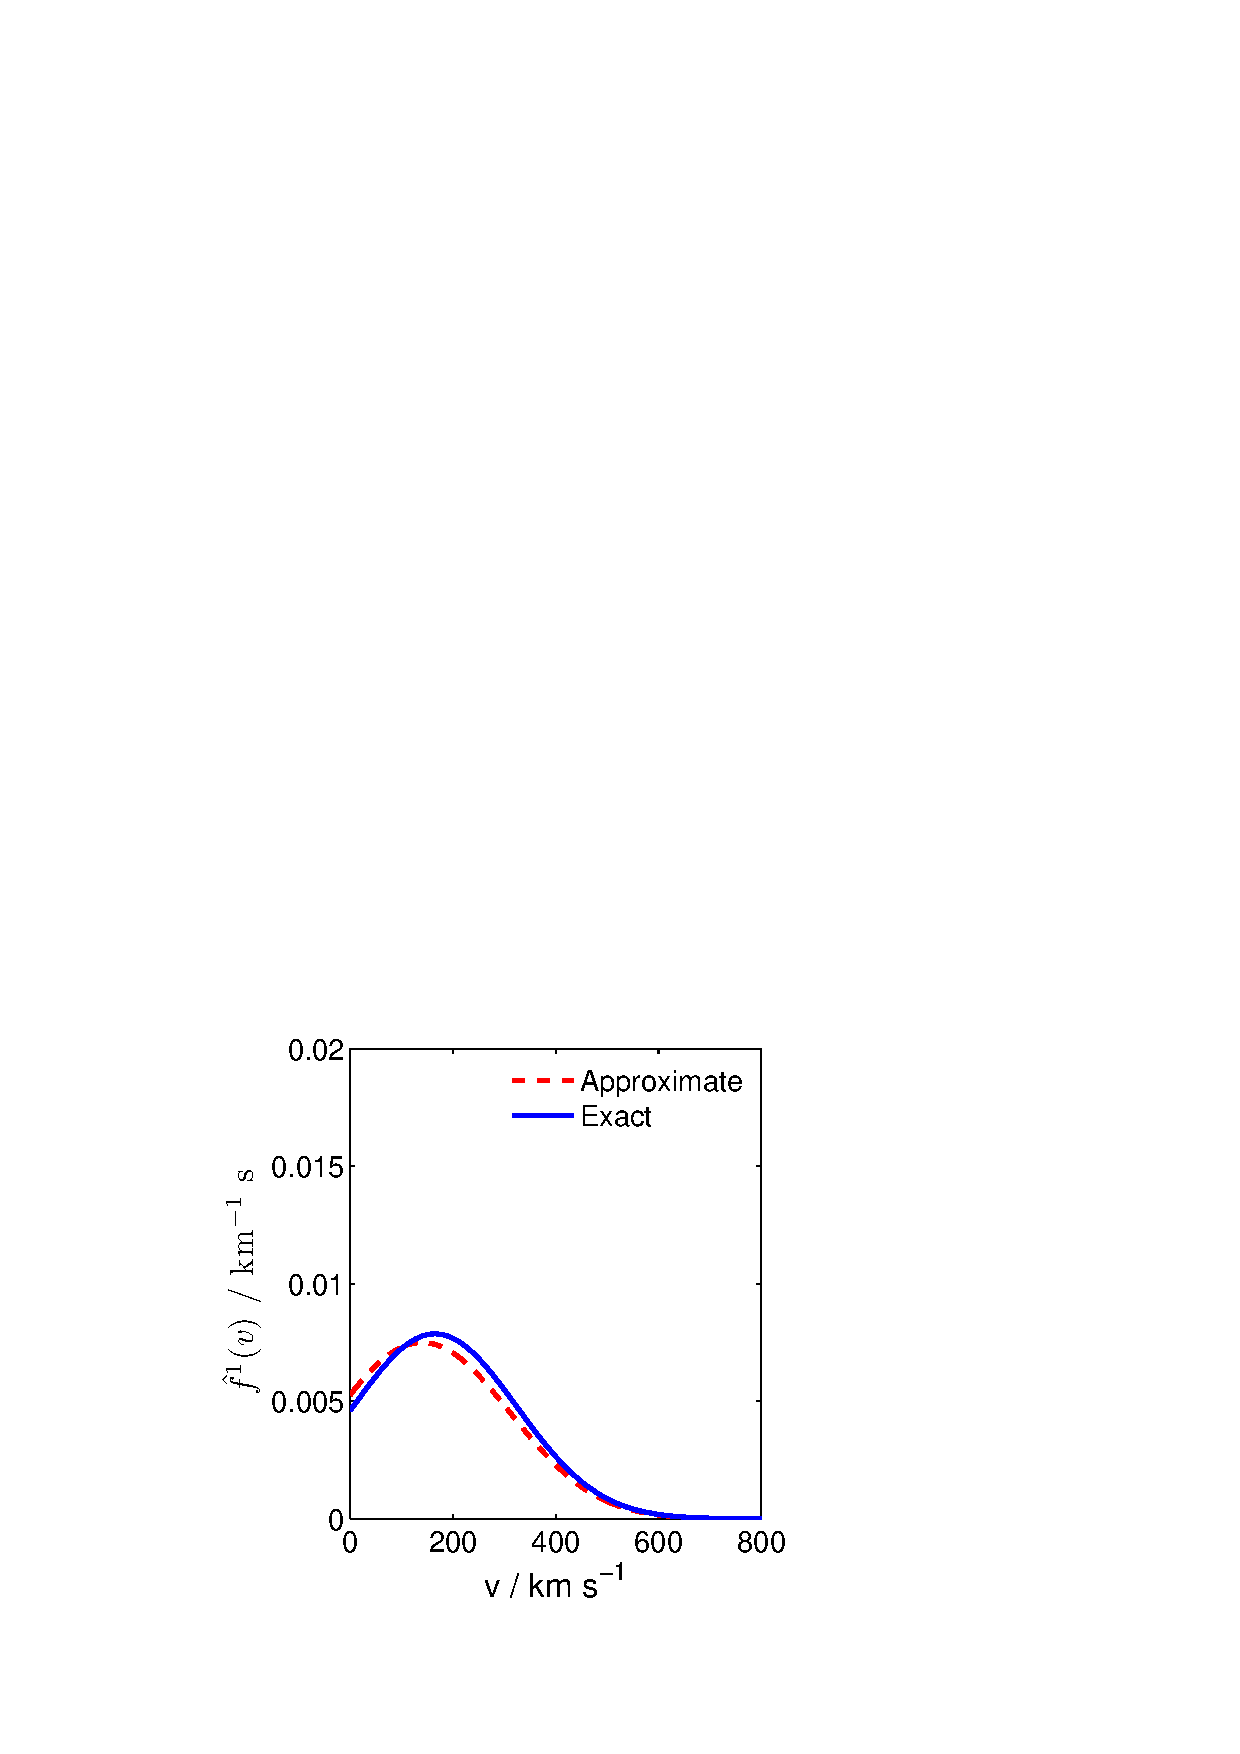
\includegraphics[trim={3.5cm 2cm 7.5cm 17cm},clip,width=0.49\textwidth]{Directional/SHM_N3_1.pdf}
  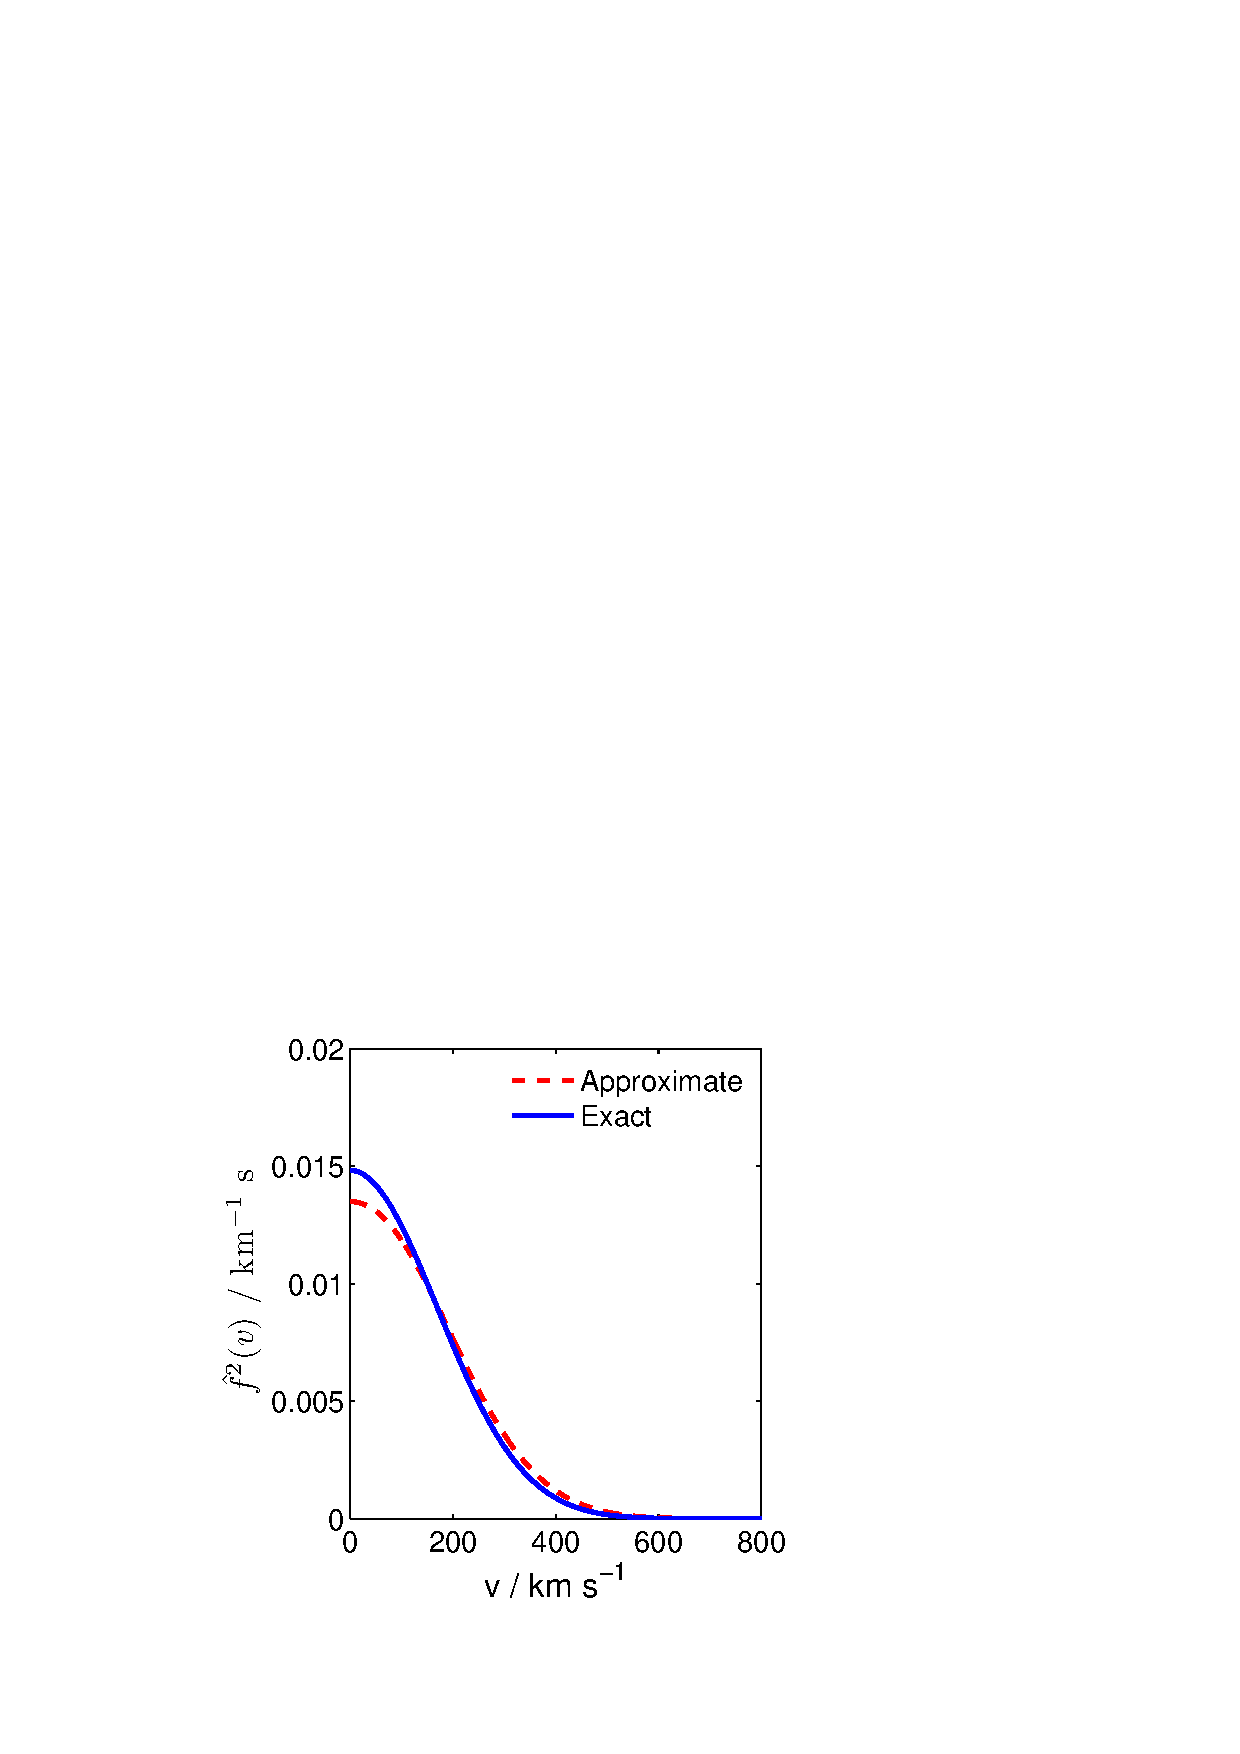
\includegraphics[trim={3.5cm 2cm 7.5cm 17cm},clip,width=0.49\textwidth]{Directional/SHM_N3_2.pdf}

  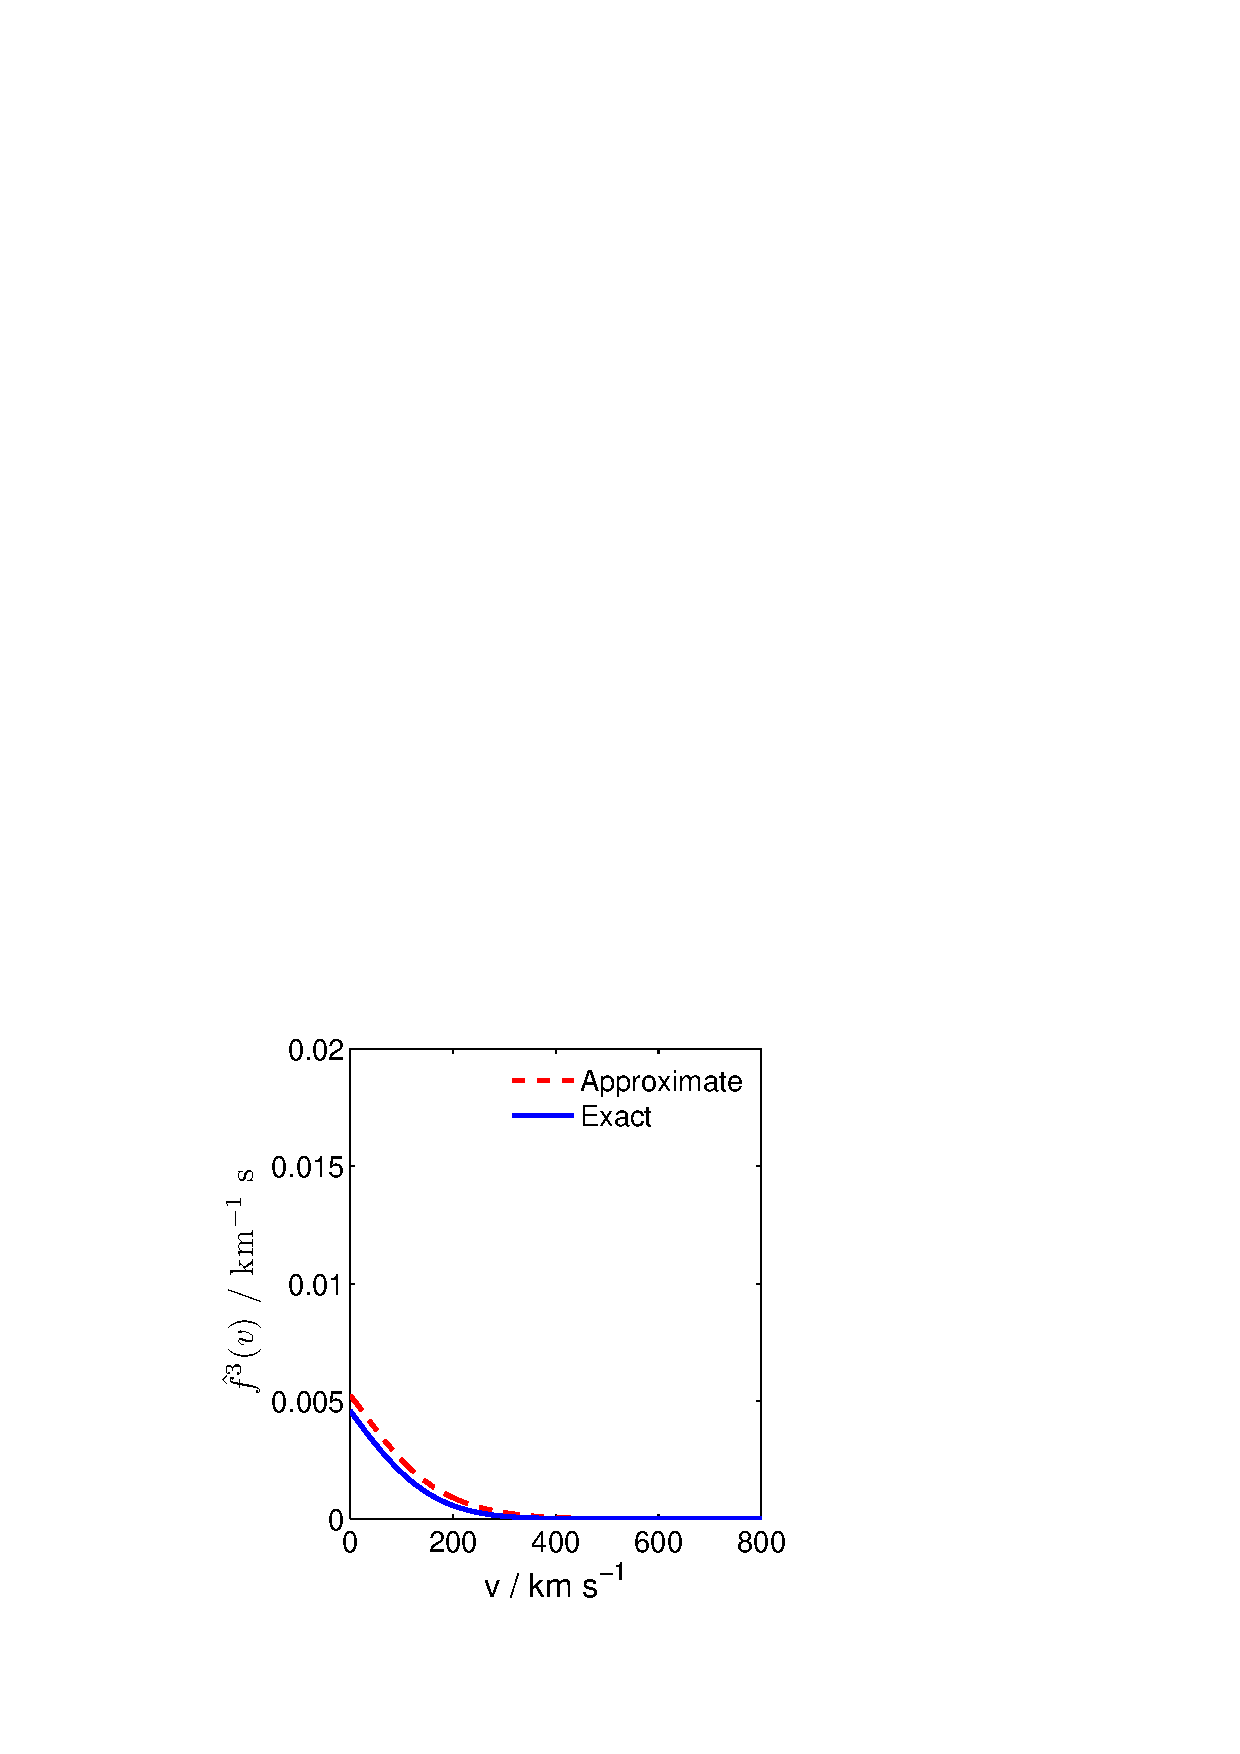
\includegraphics[trim={3.5cm 2cm 7.5cm 17cm},clip,width=0.49\textwidth]{Directional/SHM_N3_3.pdf}

\caption[Exact and approximate integrated Radon transforms for $N=3$ components in the SHM]{Exact and approximate forward, transverse and backward Radon transforms, $\hat{f}^1$, $\hat{f}^2$ and $\hat{f}^3$, for the SHM. The approximate Radon transforms are obtained by discretising the full velocity distribution into $N=3$ angular bins. The vector $\textbf{v}_\textrm{lag}$ is aligned along $\theta' = 0$.}
\label{fig:directional:radonN3_SHM}
\end{figure}

\begin{figure}[ht!]

  \centering
  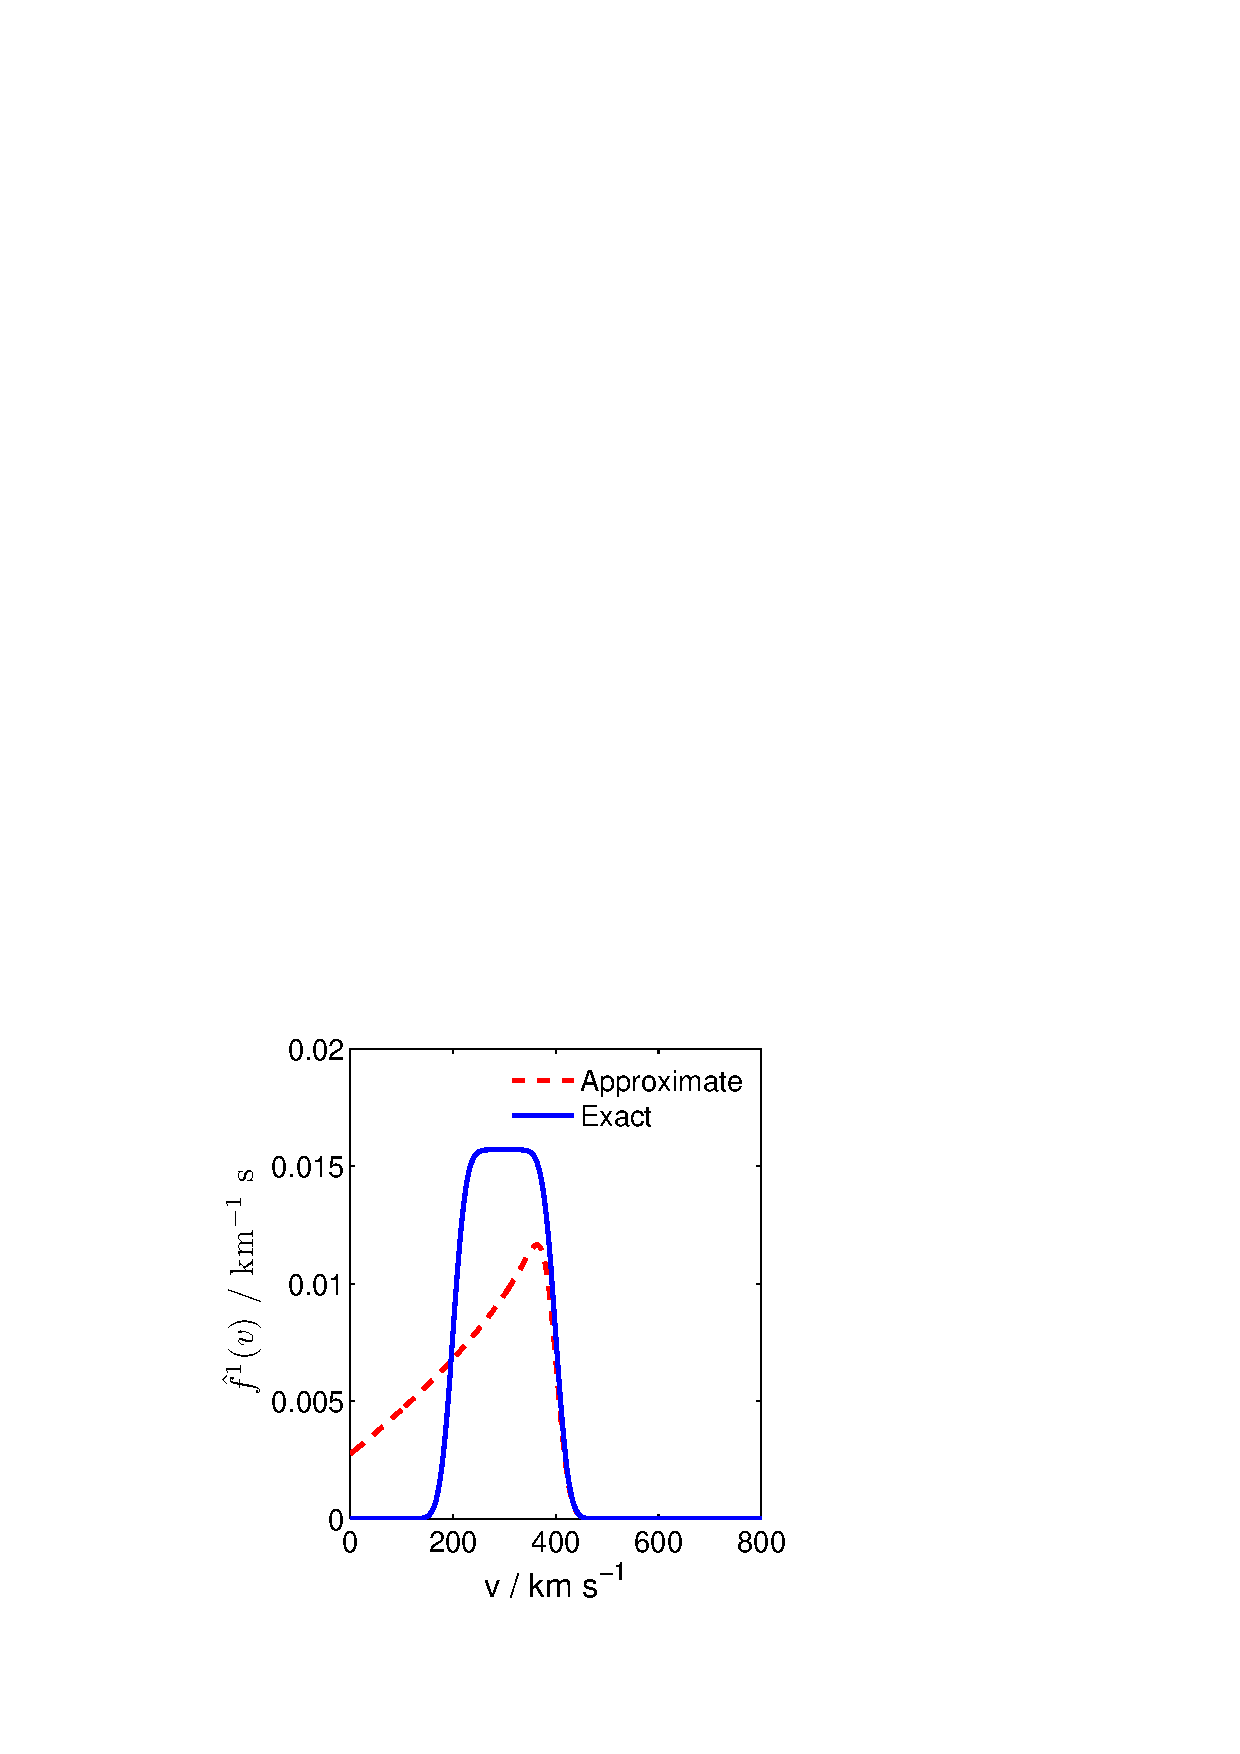
\includegraphics[trim={3.5cm 2cm 7.5cm 17cm},clip,width=0.49\textwidth]{Directional/STREAM_N3_1.pdf}
  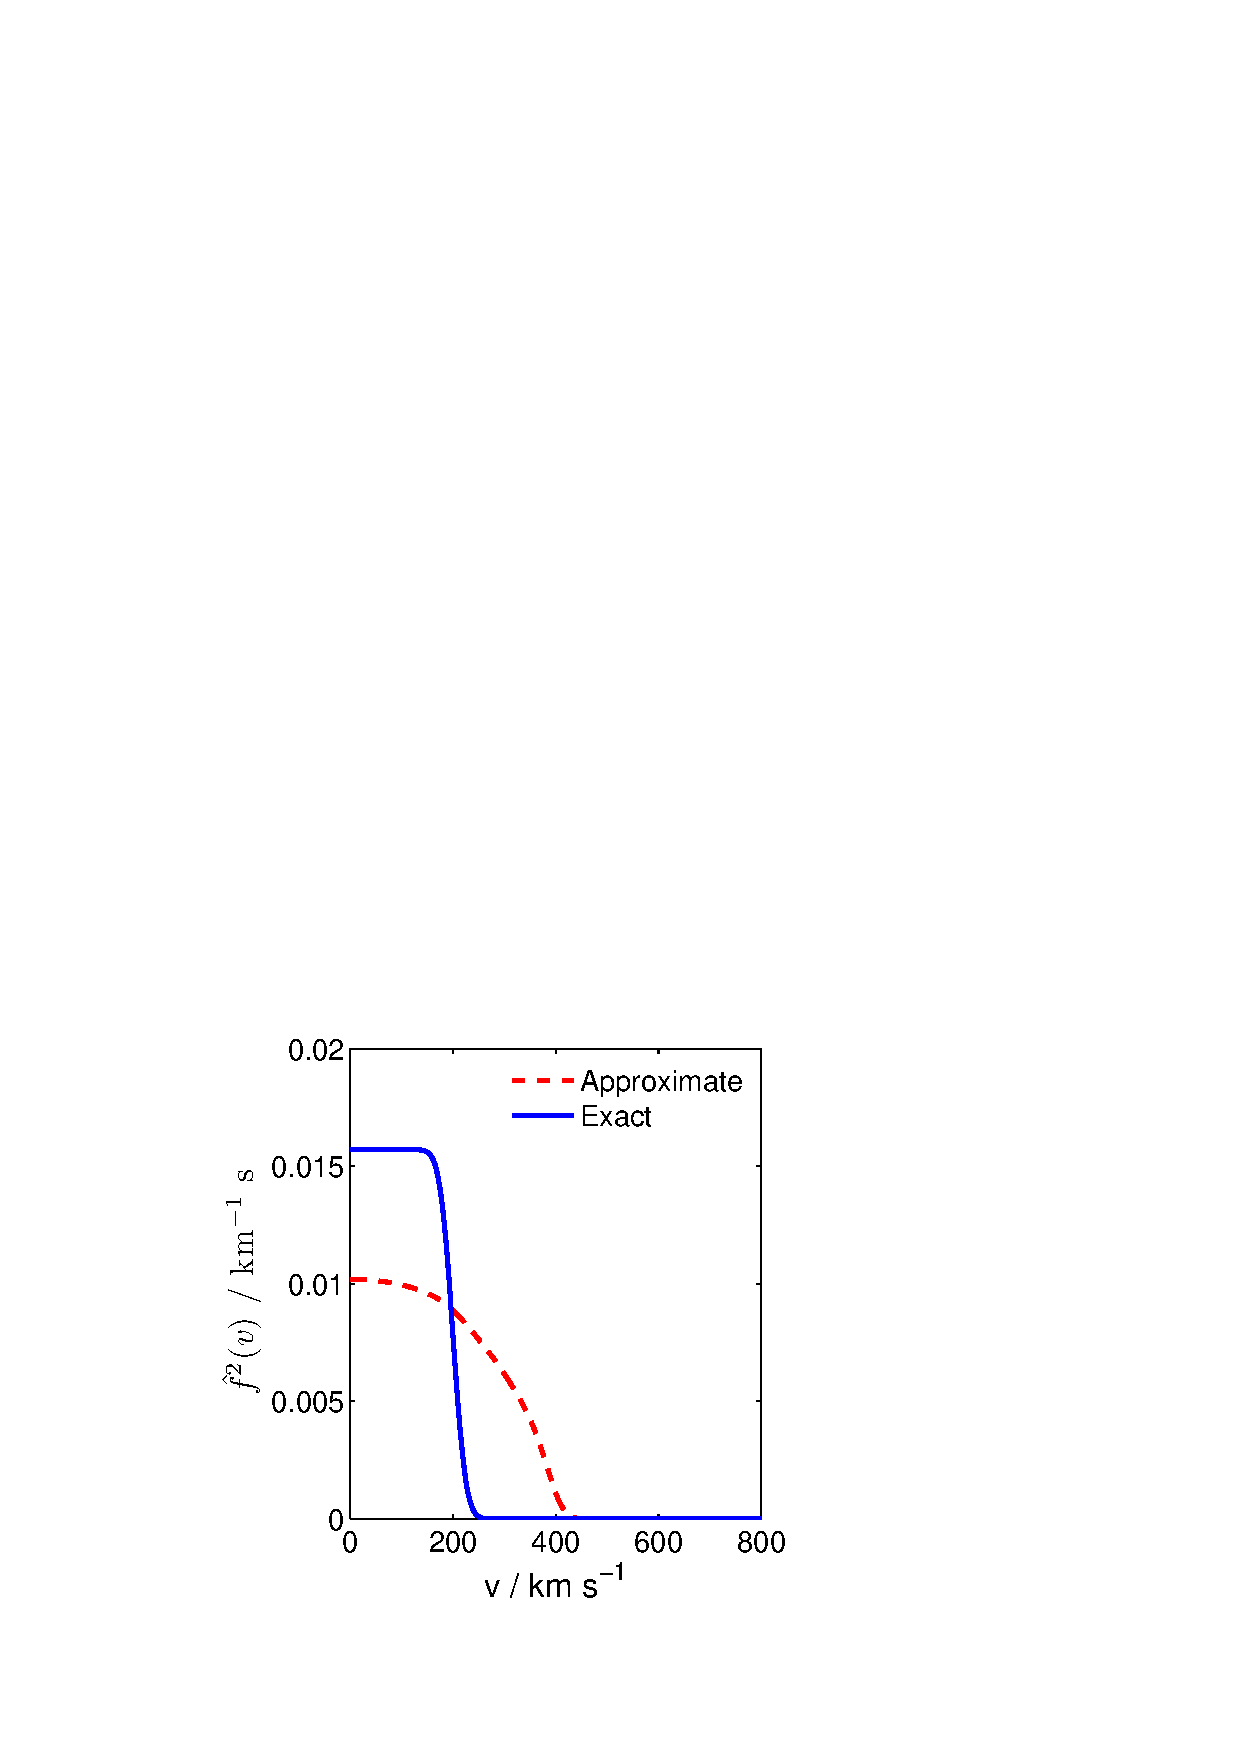
\includegraphics[trim={3.5cm 2cm 7.5cm 17cm},clip,width=0.49\textwidth]{Directional/STREAM_N3_2.pdf}

  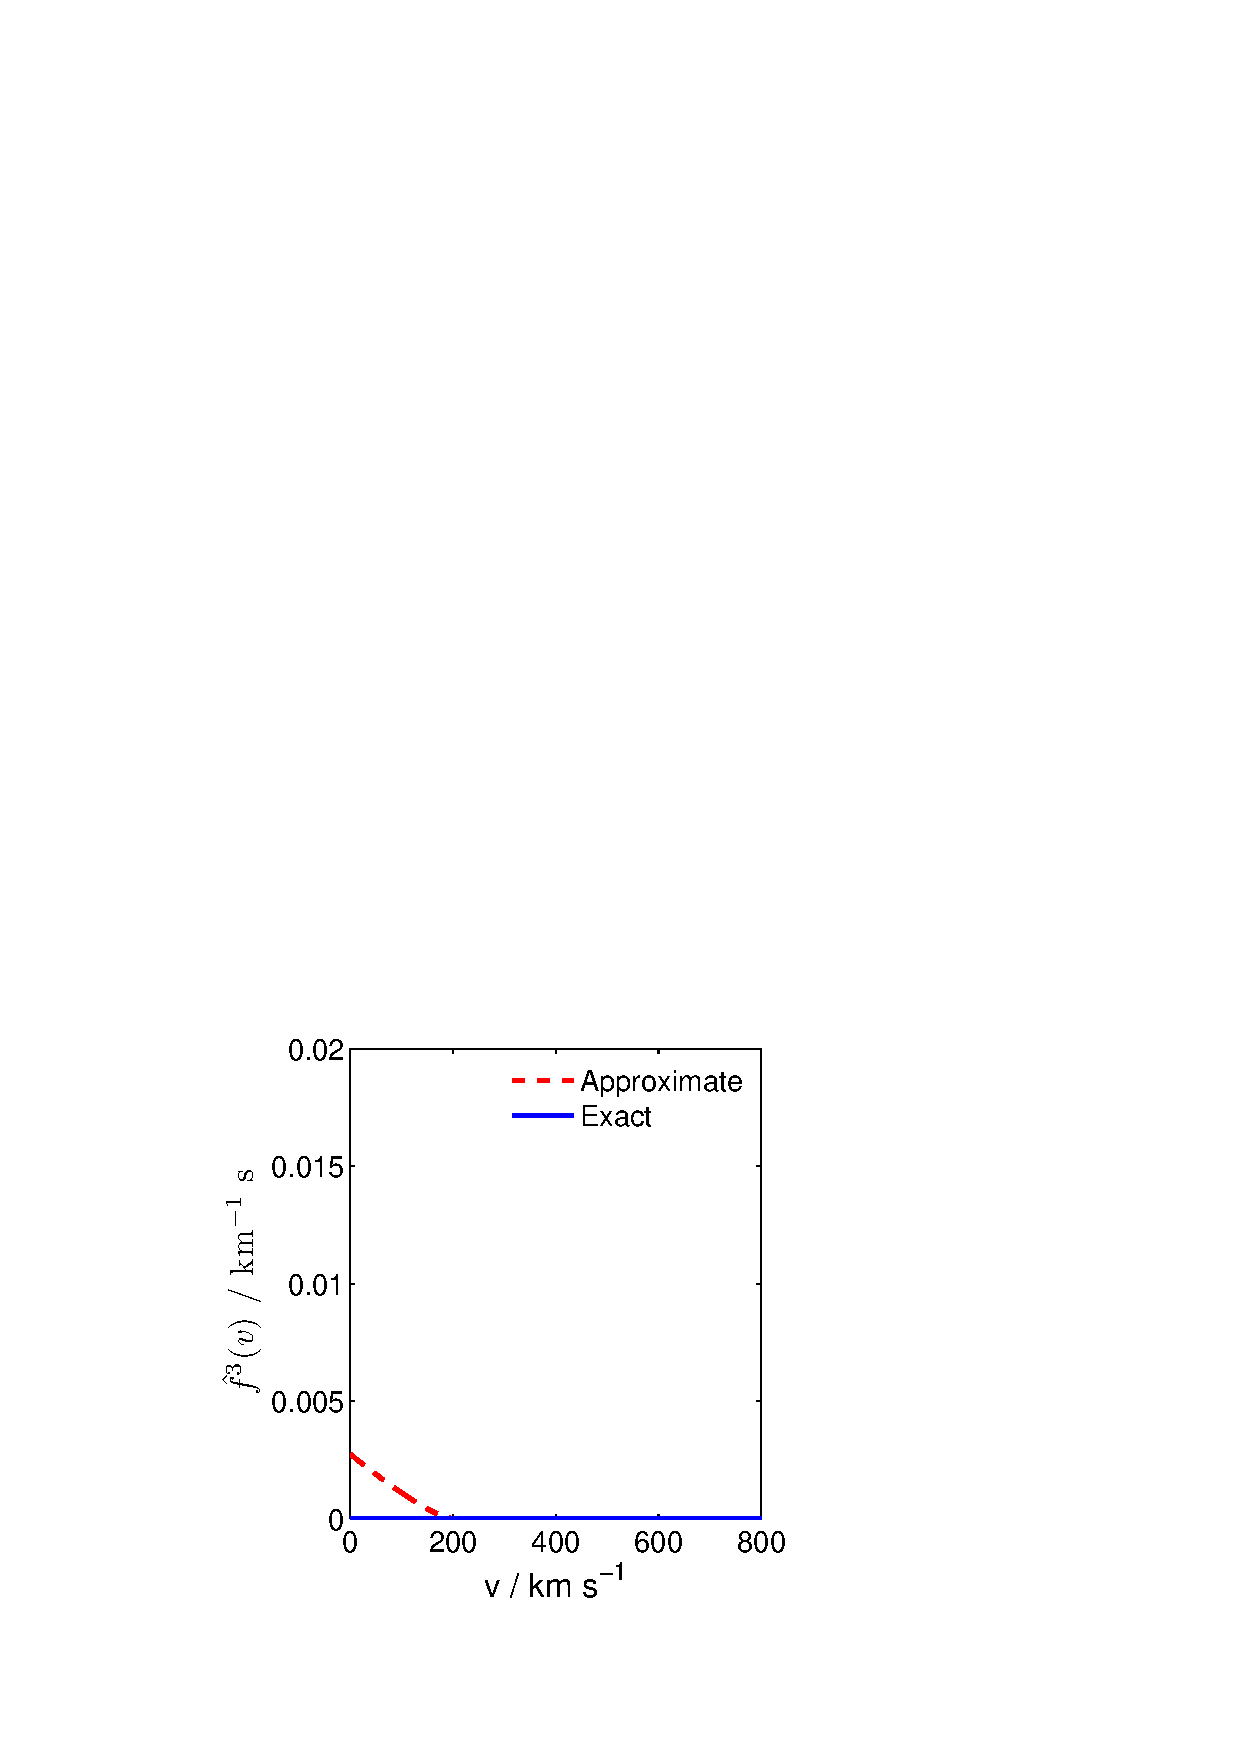
\includegraphics[trim={3.5cm 2cm 7.5cm 17cm},clip,width=0.49\textwidth]{Directional/STREAM_N3_3.pdf}

\caption[Exact and approximate integrated Radon transforms for $N=3$ components for a stream distribution function]{As Fig.~\ref{fig:directional:radonN3_SHM}, but for a stream distribution with $v_\textrm{lag} = 400 \kms$ and $\sigma_v = 20 \kms$.}
\label{fig:directional:radonN3_STREAM}
\end{figure}

\subsubsection{The folded distribution}

As discussed in Sec.~\ref{sec:directional:experiments}, sense discrimination between forward and backward-going recoils may not be possible with near-future detectors. In this case then, all that can be measured is the so called `folded' recoil spectrum

\begin{equation}
\frac{\mathrm{d}R}{\mathrm{d}E_R\mathrm{d}|\cos\theta|} = \frac{\mathrm{d}R}{\mathrm{d}E_R\mathrm{d}\cos\theta} + \frac{\mathrm{d}R}{\mathrm{d}E_R\mathrm{d}(-\cos\theta)}\,.
\end{equation}
As a result, we are concerned not with the full Radon transform of $f(\textbf{v})$, but the folded Radon transform $\hat{f}(\vmin, |\cos\theta|)$. In the case of $N=2$ discretisation, this folded Radon transform would have no directional information (because the forward and backward scattering rates differ only in the sign of $\cos\theta$). However, in the $N=3$ case, the transverse Radon transform, given by

\begin{equation}
\hat{f}^T(\vmin) = \hat{f}^2(\vmin) = \int_{-1/2}^{1/2} \hat{f}(\vmin, \cos\theta) \,\mathrm{d}\cos\theta\,,
\end{equation}
is invariant under $\hat{f}(\vmin, \cos\theta) \rightarrow \hat{f}(\vmin, -\cos\theta)$. That is, the transverse event rate `folds' back onto itself. Thus, even without sense discrimination, directional experiments will still be sensitive to this transverse scattering rate. By comparison, if the forward and backward directions cannot be distinguished, the remaining two integrated Radon transforms (the top left and bottom panels in Fig.~\ref{fig:directional:radonN3_SHM}) are folded together, to obtain the longitudinal rate
\begin{equation}
\hat{f}^L(\vmin) = \int_{-1}^{-1/2} \hat{f}(\vmin, \cos\theta) \,\mathrm{d}\cos\theta + \int_{1/2}^{1} \hat{f}(\vmin, \cos\theta) \,\mathrm{d}\cos\theta\,.
\end{equation}

We plot the transverse and longitudinal integrated Radon transforms in Fig.~\ref{fig:directional:radonN3folded} for the SHM. As expected, the two rates are now more similar in shape as we have lost some directional information. The approximate Radon transforms, obtained from the discretisation, match the true transforms closely for speeds above $\vmin\approx 200 \kms$. For a Fluorine target with a 20 keV energy threshold \cite{Daw:2011}, speeds lower than this will be below the threshold energy for all WIMP masses and the bias introduced by discrepancies at low speeds should be minimal.

\begin{figure}[t]

  \centering

  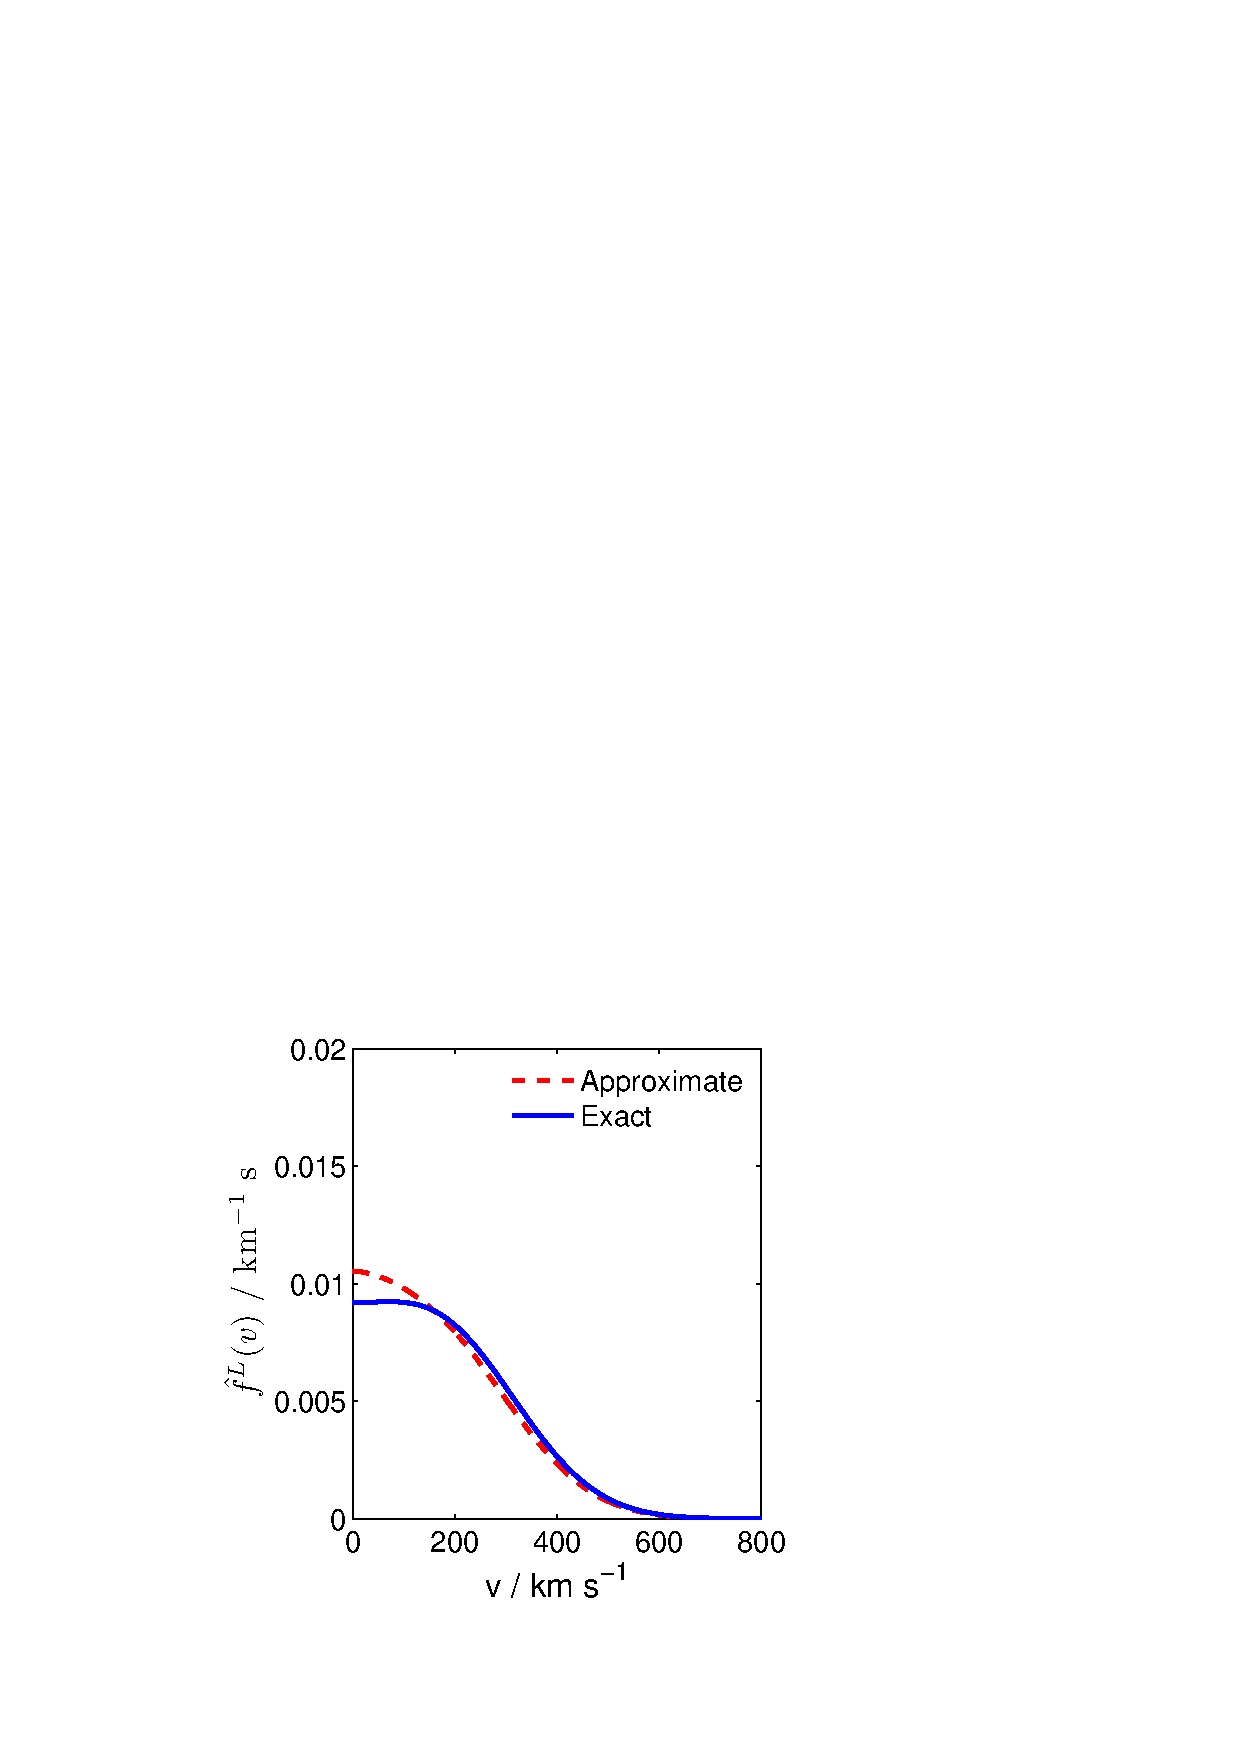
\includegraphics[trim={3.5cm 2cm 7.5cm 17cm},clip,width=0.49\textwidth]{Directional/SHMfolded_N3_L.pdf}
  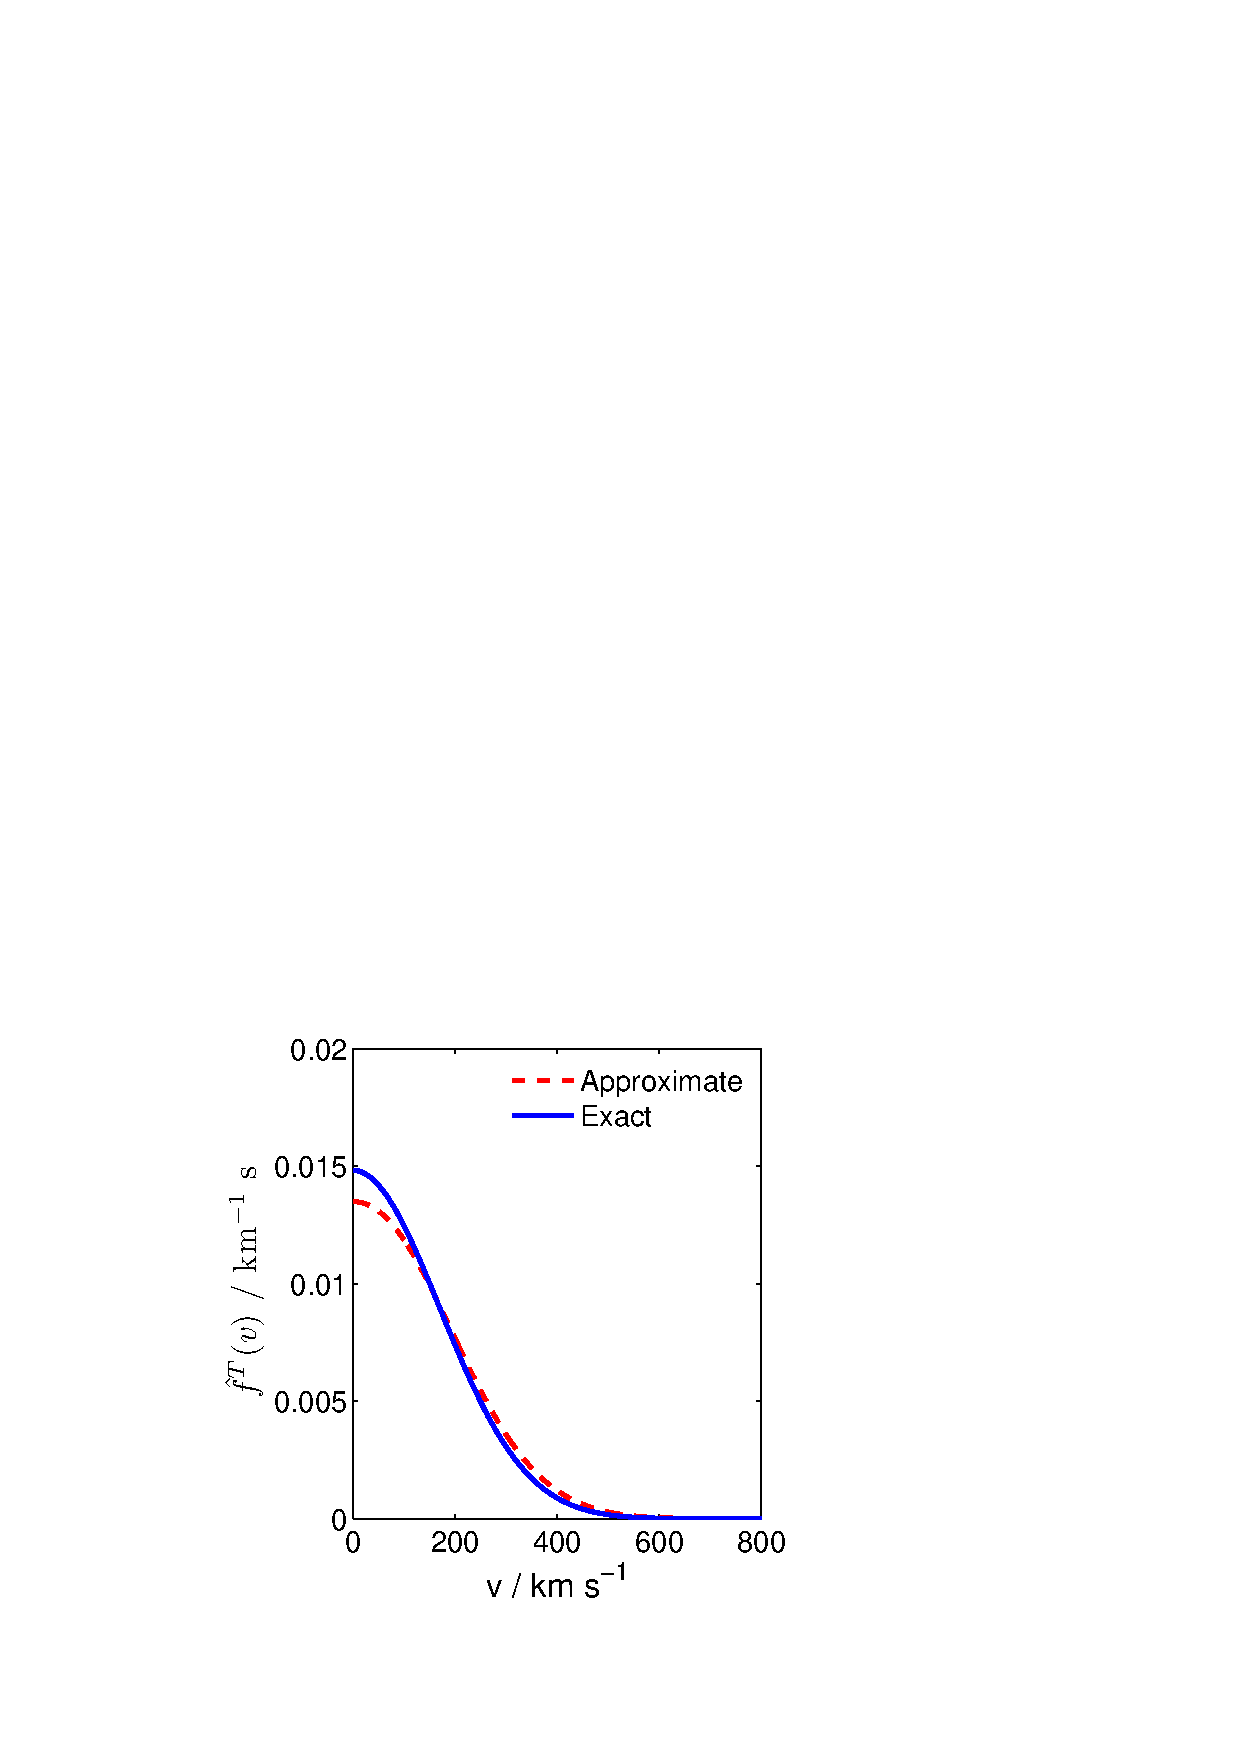
\includegraphics[trim={3.5cm 2cm 7.5cm 17cm},clip,width=0.49\textwidth]{Directional/SHMfolded_N3_T.pdf}

\caption[Exact and approximate folded Radon transforms for $N=3$ components in the SHM]{Exact and approximate folded transforms when the full SHM velocity distribution is discretised into $N = 3$ directional pieces. In the `longitudinal' case ($\hat{f}^L$) $|\cos\theta| \in [1/2,1]$ while in the `transverse case' ($\hat{f}^T$) $|\cos\theta| \in [0, 1/2]$. The vector $\textbf{v}_\textrm{lag}$ is aligned along $\theta' = 0$.}
\label{fig:directional:radonN3folded}
\end{figure}

We note that in this folded case, we would fit to two data sets, corresponding to the longitudinal and transverse event rates. However, our original discretisation required 3 free functions of $v$: $f^{1,2,3}(v)$. However, due to the properties of the Radon transform, the longitudinal rate is not a function of $f^1(v)$ and $f^3(v)$ but of the sum $f^1(v) + f^3(v) \equiv f_L(v)$. Thus, we have only two free functions $f^{L,T}(v)$ to fit.


\section{Discussion}

We have demonstrated that for smooth SHM-like distributions, the discretised velocity distribution allows us to obtain a good approximation to the discretised Radon transform. This means that we should be able to parametrise the speed distributions in each angular bin $f^k(v)$ and account for astrophysical uncertainties without introducing a large error in the recoil spectrum.
An additional dark disk contribution would further reduce the error between the exact and approximate Radon transforms, as the dark disk is expected to approximately corotate with the Earth and would thus appear more isotropic than the SHM. However, strongly peaked velocity distributions, such as the stream studied in the previous sections, would introduce a much larger error in the Radon transform. While such distributions are not considered likely (see Sec.~\ref{sec:DD:astrounc}), we should bear in mind that a larger value of $N$ may be required for these more extreme distributions.

The decomposition we have presented in this chapter is coordinate dependent (as is a spherical harmonic decomposition). That is, we must specify which direction corresponds to $\theta' = 0$. In a real experiment, we would want to choose this direction to maximise the directional signal, in order to obtain the most information from the data. Therefore, we would ideally like to choose $\theta' = 0$ along the direction of the mean WIMP velocity. In the SHM, this is parallel to $\mathbf{v}_\textrm{lag}$, which corresponds to the direction of the Earth's motion in the Galactic frame, which has been calculated \cite{McCabe:2014}. It might also be possible to use the median recoil direction to determine the mean WIMP velocity and thereby fix $\theta'$. We note that for the results presented in this chapter we have fixed $\theta' = 0$ parallel to $\mathbf{v}_\textrm{lag}$. If we instead choose a different direction for $\theta'= 0$, this would decrease the forward-backward asymmetry of the discretised velocity distribution, reducing the error between the exact and approximate Radon transforms. Thus, the results presented would not be spoiled by a different choice of $\theta'$.

Another consideration we have not yet addressed is the fact that in an experiment, we measure the directional recoil spectrum, not the Radon transform. Thus, we must multiply by the appropriate form factor and apply realistic thresholds in order to apply the methods presented here to directional data. Perhaps more important, however, is finite angular resolution. As discussed in Sec.~\ref{sec:directional:experiments}, directional detectors have angular resolutions of 20$\,^{\circ}$-80$\,^{\circ}$. In future work, this should be taken into account to determine the true directional recoil spectrum measured in an experiment. This angular smoothing will make the measured spectrum less anisotropic which again should reduce the error induced by considering a discretised velocity distribution.

Finally, in order to accommodate more strongly peaked distribution functions (or to obtain more directional information as the amount of data increases), it will be necessary to considered discretised distributions with $N > 3$. In future, we must develop an algorithm for generating the discrete Radon transforms from discrete velocity distributions of arbitrary $N$. As outlined in Appendix~\ref{ch:RadonCalc}, the angular integrals can be performed explicitly for any value of $N$, leaving only a series of 1-dimensional integrals over elementary functions of the WIMP speed $v$. Thus, it should be possible to extend this framework to arbitrary $N$ without requiring any (potentially slow) numerical integration over the angular variables.

\section{Conclusions}

Directional direct detection experiments should allow us to probe the full WIMP velocity distribution. However, as in the non-directional case, this introduces significant uncertainties into the analysis of data. Parametrising the velocity distribution and therefore reconstructing its structure requires a very large number of parameters, as $f(\mathbf{v})$ is a function of the 3-dimensional vector $\mathbf{v}$. It is therefore necessary to decompose $f(\mathbf{v})$ into some angular basis and parametrise the corresponding coefficients. Previous attempts in this direction have required equilibrium assumptions about the Galactic halo, or have made use of a spherical harmonic basis. An expansion in this basis does not necessarily lead to a physical distribution function, as it does not ensure that $f(\textbf{v})$ is everywhere positive.

We have presented an alternative decomposition of $f(\textbf{v})$ into angular bins. Over each bin, the velocity distribution has no angular dependence. As long as the parametrisation for the radial part of $f(\mathbf{v})$ is everywhere positive, so too will be full velocity distribution. We have demonstrated how the corresponding binned Radon transforms can be calculated for the case of $N=1,2,3$ and compared these with the exact Radon transforms obtained from the full distribution.

In the $N=2$ case, the discretised approximation underestimates the forward rate and overestimates the backward rate. However, this is improved in going to the $N=3$ case, for which the exact and approximate Radon transforms agree to within 10-15\%. For $N=3$, it should also be possible to extract directional information even when sense recognition is not possible. For a more sharply peaked distribution, such as a stream, the error induced by using the discretised velocity distribution is significant. It would therefore be necessary to go to higher values of $N$ in order to capture the strongly anisotropic features of such a distribution.

We have presented here a framework for parametrising the directional part of the velocity distribution. In future, it will be necessary to test this method using mock data from directional detectors in order to determine how well the WIMP parameters and the distribution itself can be reconstructed. This will require us to determine the mean WIMP direction, as well as to include realistic experimental effects, such as angular resolution. However, we have argued that the good agreement between the exact and approximate rates for the case of smooth distributions should not be spoiled by these effects. Finally, it will be necessary to extend this framework to higher values of $N$ to capture more angular information if larger numbers of events are observed at directional detectors.


